\documentclass[12pt]{article}
%\usepackage{scicite}
%\usepackage{times}
\usepackage{pdfpages}
\author{Aaron Spring}
%\usepackage[ansinew]{inputenc}
\usepackage{amsmath}
\usepackage{siunitx}
\usepackage[colorlinks=true, urlcolor=blue, linkcolor=darkgray,citecolor=blue]{hyperref}
%\usepackage[german]{babel}
\usepackage{float}
%\usepackage[numbers]{natbib}
\usepackage[authoryear]{natbib}
%\usepackage[pliannatuthoryear]{natbib}
\usepackage{indentfirst}
\usepackage{amsmath}
%\renewcommand{\vec}[1]{\boldsymbol{#1}}

\usepackage{chngcntr}
\usepackage{pinlabel}
\usepackage{graphicx}
\graphicspath{{/home/mpim/m300524/MSc_Thesis/gfx/}}

% The following parameters seem to provide a reasonable page setup.

\topmargin 0.0cm
\oddsidemargin 0.2cm
\textwidth 16cm 
\textheight 21cm
\footskip 1.0cm

%\newcommand{\memberpositive}{m105_1994_2001}
\newcommand{\memberpositive}{m178_1985_1992} %funktioniert am besten
%\newcommand{\memberpositive}{m182_1988_1995} % zweitbesten


%\newcommand{\membernegative}{m113_1986_1993}
\newcommand{\membernegative}{m143_1995_2002}
\allowdisplaybreaks


%The next command sets up an environment for the abstract to your paper.

%\newenvironment{sciabstract}{%
%\begin{quote} \bf}
%{\end{quote}}


% If your reference list includes text notes as well as references,
% include the following line; otherwise, comment it out.

\renewcommand\refname{References and Notes}

% The following lines set up an environment for the last note in the
% reference list, which commonly includes acknowledgments of funding,
% help, etc.  It's intended for users of BibTeX or the {thebibliography}
% environment.  Users who are hand-coding their references at the end
% using a list environment such as {enumerate} can simply add another
% item at the end, and it will be numbered automatically.

%\newcounter{lastnote}
%\newenvironment{scilastnote}{%
%\setcounter{lastnote}{\value{enumiv}}%
%\addtocounter{lastnote}{+1}%
%\begin{list}%
%{\arabic{lastnote}.}
%{\setlength{\leftmargin}{.22in}}
%{\setlength{\labelsep}{.5em}}}
%{\end{list}}

\setcounter{tocdepth}{2}


\begin{document} 

% Double-space the manuscript.

\baselineskip24pt

% Make the title.
%\title{Internal variability of the Southern Ocean carbon sink in MPI-ESM large ensemble simulations} %\\ assessment of westerly wind changes}
\title{Decadal variations in the Southern Ocean carbon sink in MPI-ESM 100 ensemble simulations} %\
\maketitle 
%\Huge
\vspace{5cm}
\begin{center}
\Huge
\textbf{Outline}
\end{center}

\normalsize
\newpage
\tableofcontents

\newpage

\section{Introduction}

\paragraph{Why the Southern Ocean is important} 
The oceans are major carbon sink by taking up about 25-30\% of the anthropogenic carbon emissions from the atmosphere \citep{Quere2016}. As a key region, the Southern Ocean contributes about 40\% to the global ocean carbon sink \citep{Sabine2004}. Due to the sparse spatial and temporal coverage in the Southern Ocean, various observational CO$_2$ flux products yield large uncertainties \citep{Roedenbeck2015}. Also modeling results have a large spread \citep{Wang2016}, but claim the Southern Ocean as a constraint to reduce model uncertainties \citep{Kessler2016}.

\paragraph{Southern Ocean observations and demand for models}
Recent observations suggest pronounced decadal variations in the Southern Ocean carbon sink \citep{Roedenbeck2013,landschuetzer2015}. However, due to the sparse spatial and temporal coverage, it is challenging to discern the dynamics of internally varying processes, which demands for the evaluation with models. Earth system models (ESMs) are a useful tool to analyze processes that contribute to variability. \cite{Lovenduski2007,Lovenduski2008} explained the mechanistic processes behind the positive trend in the Southern Annular Mode with a ocean model with atmospheric forcing from reanalysis data. Yet, ESMs, containing a freely evolving coupled atmospheric and ocean component, don't capture the decadal variations suggest by observations \citep{Wang2016}. Using a large ensemble of simulations with perturbed initial conditions but identical forcing and model allows to separate the forced signal and internal variability.

\paragraph{What I do and research questions}
By using a large ensemble simulation based on the Max-Planck-Institute Earth System Model (MPI-ESM), I investigate the variability of the oceanic carbon uptake. I try to answer the following reseach questions: 
\begin{itemize}
\item What is the modeled internal variability of the Southern Ocean carbon sink? 
\item How does variability in biological and physical processes influence the carbon sink?
\end{itemize} 


 
%why did Tatiana want me to do this:
%all coupled models fail to reproduce SO variability, ocean-only models with NCEP forcing catch it, so its probably the winds and need coupled ensemble simulation
 
\paragraph{Working hypothesis}
The Southern Annular Mode (SAM), characterizing the strength and position of the westerly winds, is known to be the dominant mode of climate variability in the Southern hemisphere \citep{Thompson2000,Thompson2011}.  Supposing the strength and position of the westerlies winds as the major reason for climate variability for the Southern Ocean \citep{Thompson2000}, how does the carbon system respond? Changes in westerly winds alter circulation patterns, which directly effect the carbon sink via the thermal effect, circulation of carbon and biological production.

\paragraph{Revisit processes}
In this thesis, I revisit the dominant processes leading to extreme trends in the Southern Ocean carbon sink in the biogeochemical model HAMOCC [similar \cite{Lovenduski2007,Lovenduski2008}, as individual processes related to changes in winds are already discussed for changes in temperature \citep{Takahashi1993,Lovenduski2007}, circulation \citep{Abernathey2011,Hauck2013,Lauderdale2016,Lovenduski2008} and biology \citep{Lovenduski2005,Tagliabue2014,wang2012}. This revisit is particularly interesting as other large ensembles of perturbed initial conditions do not capture strong decadal variations in the Southern Ocean carbon sink whereas MPI-ESM LE does [private communication N. Lovenduski (NCAR) and S. Schlunegger (GFDL), see section \ref{sec:PICLE} for details].



\clearpage

\section{Methods}

\subsection{Model description of the MPI-ESM}

%preamble: 
%\paragraph{Model components} 
The Max-Planck-Institute for Meteorology Earth System Model (MPI-ESM) 
consists of coupled general circulation models of the atmosphere ECHAM6 \citep{Stevens2013} and ocean MPIOM \citep{Jungclaus2013} as well as subsystem models for vegetation on land JSBACH \citep{Reick2013} and for marine biogeochemistry HAMOCC \citep{Ilyina2013}. The large ensemble simulations are based on MPI-ESM version 1.1.00p2 \footnote[1]{full source code: \url{https://code.zmaw.de/projects/mpi-esm/repository/show/tags/mpiesm-1.1.00p2}} with a low-resolution configuration. Since the atmospheric pCO$_2$ levels are prescribed, terrestrial carbon cycle from the land component JSBACH and oceanic carbon cycle from HAMOCC do not interact (fig. \ref{fig:MPIESM}). The full earth-system model \citep{Giorgetta2013} as well as its components have been described and evaluated in detail by the given references. In the following subsections, I give an overview about the implemented processes affecting internal variability of the oceanic carbon cycle.



%The Max-Planck-Institute for Meteorology Earth System Model (MPI-ESM) version 1.1.00p2 \footnote[1]{full source code: \url{https://code.zmaw.de/projects/mpi-esm/repository/show/tags/mpiesm-1.1.00p2}} with a low-resolution configuration is used for the large ensemble simulations \citep{Giorgetta2013}. The atmosphere component ECHAM6.3 runs on a T63 grid, corresponding to 1.9$^\circ$ horizontal resolution, with 47 vertical layers up to 0.01 hPa \citep{Stevens2013}. The ocean component MPI Ocean Model (MPIOM) has a horizontal resolution of 1.5$^\circ$ on average and 40 fixed-depth vertical levels \citep{Jungclaus2013}. The Hamburg Ocean Carbon Cycle Model (HAMOCC) represents the ocean biogeochemistry component (fig. \ref{fig:HAMOCC}) \citep{Ilyina2013}. Since there is no biogeochemical riverine exchange, terrestrial carbon cycle from JSBACH \citep{Reick2013} and oceanic carbon cycle do not interact (fig. \ref{fig:MPIESM}). 

\begin{figure}[h!]
	\centering 
	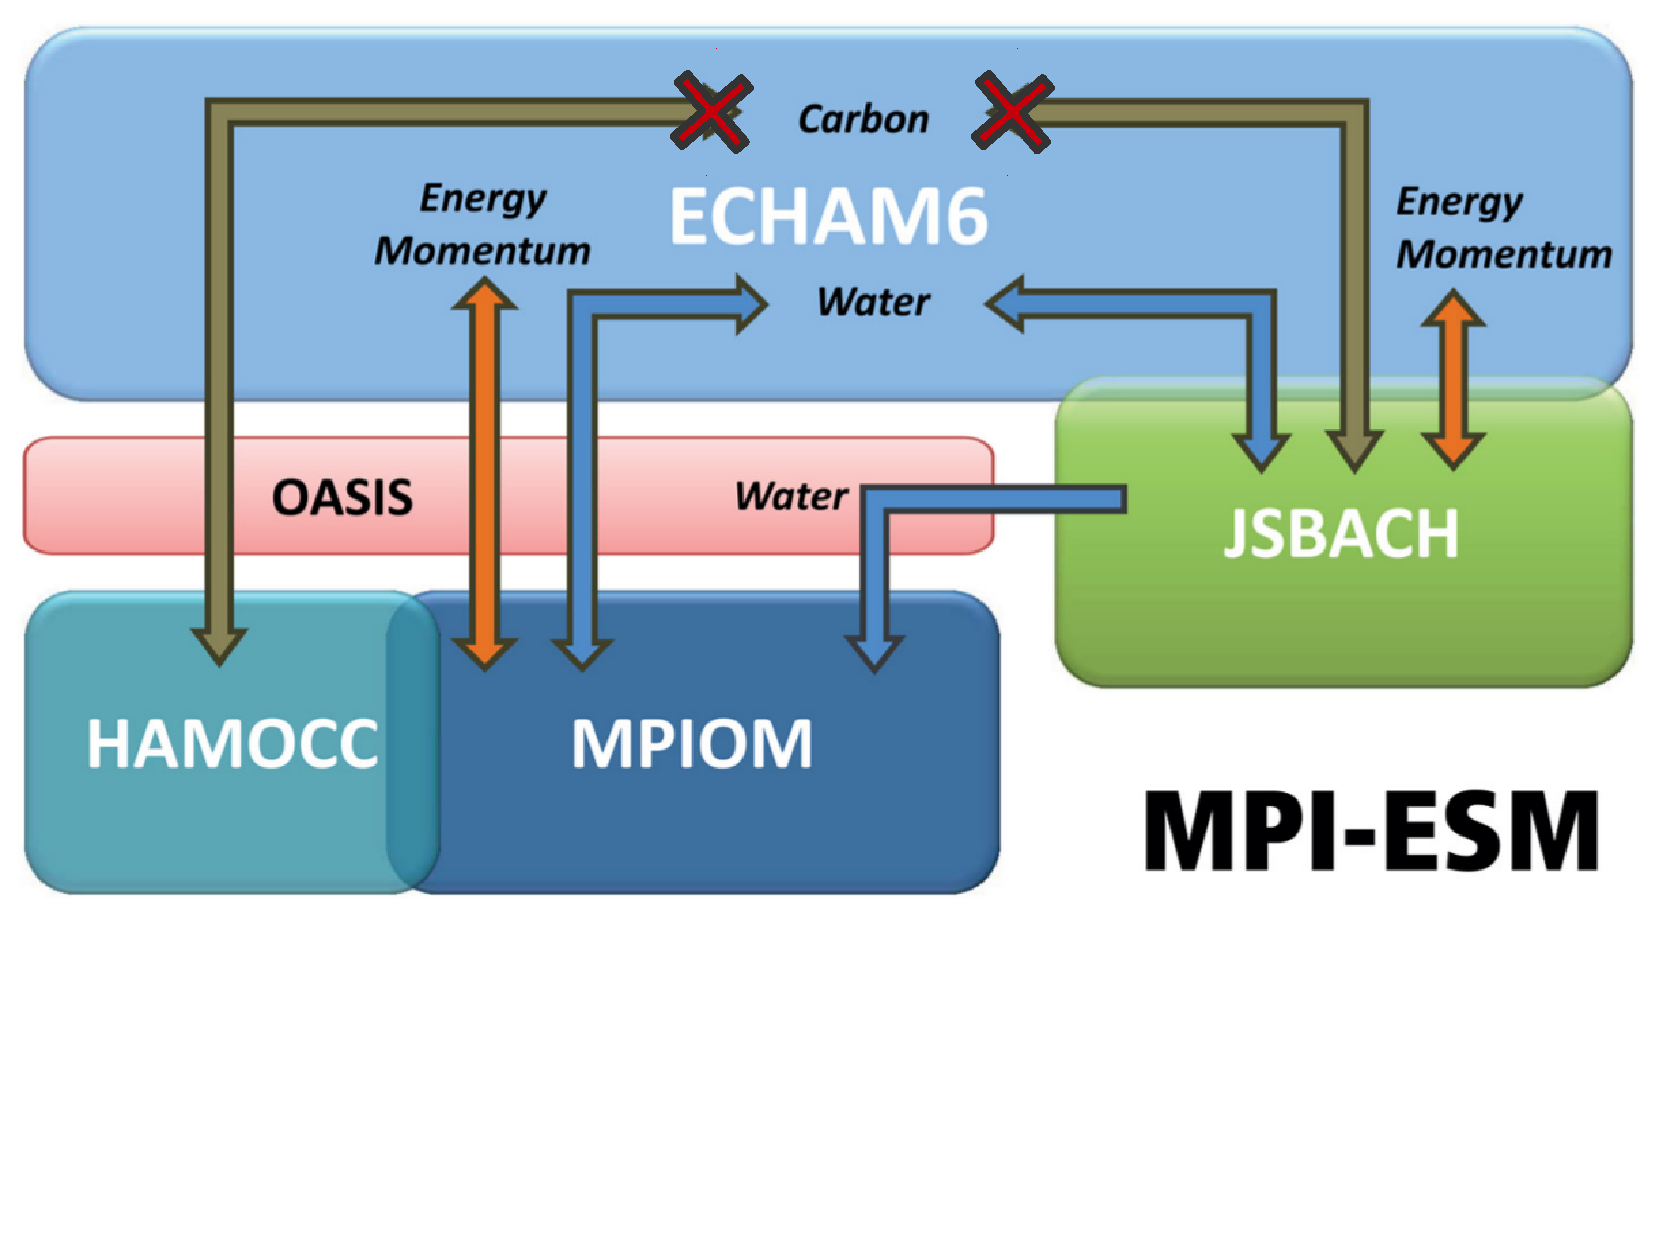
\includegraphics[scale=.57,trim=0cm 5.87cm 0cm 0cm,clip]{MPIESM.pdf}
	\caption{Schematic overview on the different components in MPI-Earth-System-Model with a non-interactive carbon cycle \citep{Giorgetta2013}}
	\label{fig:MPIESM}
\end{figure}

%\subparagraph{Note: I briefly explain how processes affecting the carbon cycle/my study are implemented and subject to internal variability}


\subsubsection{ECHAM}
ECHAM - a naming combination of European Center (EC) for Medium Range Weather Forecasts (ECMWF) and HAM for Hamburg -  is an general circulation model for the atmoshpere. ECHAM has an air-sea gas exchange interface with HAMOCC and exchanges water, energy and momentum with MPIOM. 
The atmosphere component ECHAM6.3 runs on a T63 grid, corresponding to 1.9$^\circ$ horizontal resolution, with 47 vertical layers up to 0.01 hPa \citep{Stevens2013}. 
This high vertical resolution and atmospheric height allows to model jets which originate in the tropopause. Those jets define the position and strength of the westerly winds in the Southern hemisphere.  In ECHAM extratropical jets are slightly shifted to lower latitudes \citep{Stevens2013} which seems to be a common atmospheric modeling challenge \citep{Kidston2010}.
Changes in ECHAM with regard to CMIP5 version in \cite{Stevens2013} are described in \cite{Bittner2016}. They majorly include a new radiation code of ECHAM6.3 which leads to small changes in the temperature fields.  


\subsubsection{MPIOM}
\label{sec:mpiom}
%\subparagraph{relevant MPIOM info: upwelling/advection/mixing}
The ocean model MPIOM is an ocean general circulation model (OGCM) with a horizontal resolution of 1.5$^\circ$ on average on the Arakawa C-grid, 40 fixed-depth vertical levels on a realistic topography and with a free surface \citep{Jungclaus2013}. All biogeochemical and physical tracers except for opal and calcite shells are advected by the Navier-Stokes equations with Boussinesq-approximation \citep{Marsland2003}. In areas of large scale upwelling - such as the Southern Ocean - those tracers are advected to the ocean surface. Those carbon-rich waters then equilibrate with atmospheric pCO$_2$. Upwelling processes are largely driven by divergence due to winds. Strong ocean currents lead to eddies which additionally mix the water column horizontally and vertically. The spatial resolution of 1.5$^\circ$ translated to a grid cell length of $\sim$150 km at the northern edge of the Southern Ocean at 30$^\circ$S and $\sim$40 km in Antarctic coastal waters. These length scales are too small to resolve eddies, so they are parametrized by the GM-scheme \citep{Gent1995}. Therefore, the vertical mixing and diffusion based on Richardson-number dependent formulation is important for vertical gradients \citep{Pacanowski1981}. The impact of eddies on the carbon cycle, especially in the Southern Ocean, is under current research \citep{Lauderdale2013,Dufour2013,Gnanadesikan2015}.

The mixed-layer depth is calculated by a potential density criterion where the difference between the sea-surface density and the lower end of the mixed-layer is 0.125 kg m$^{-3}$ \citep{Jungclaus2013}. 




\subsubsection{HAMOCC}
\label{sec:HAMOCC}
%\subparagraph{HAMOCC coupling} 
%HAMOCC is coupled to ECHAM6 for exchange of atmoshperic gases, precipitation and energy, e.g. heat as radiation and mechanical energy as wind stress. The required state variables required for HAMOCC, such as sea-ice cover, temperature T, salinity S and advective velocities $\vec{v}$, are provided from MPIOM. 
The Hamburg Ocean Carbon Cycle model HAMOCC is a global marine carbon cycle model which simulates oceanic carbon and nutrient cycles \citep{Maier-Reimer1984,Maier-Reimer1993,Six1996}. It aims to reproduce distributions of biogeochemical parameters over various timescales from seasons to millenia without regional tuning or temporal adjustments towards observations. This includes processes on three compartments: air-sea interactive at the sea surface, biogeochemistry of the water column and sediment biogeochemistry (fig. \ref{fig:HAMOCC}). The HAMOCC model version for the large ensemble is identical to the one used in CMIP5 which is analyzed in detail in \cite{Ilyina2013}. In the following subsection, I can only give an overview about the most relevant processes for the variability on decadal and shorter timescales.

\subparagraph{CO$_2$ flux description}
The CO$_2$ flux calculation implemented in the model follows an empirical relationship under the conceptual one-layer ocean-sided stagnant film model with gas transfer velocity $k_w$ \citep{Wanninkhof1992}: 
\begin{align*}
\text{CO}_2\text{flux} &= (1-f)k_w \Delta \text{pCO}_2 \\
				k_w &= 0.31 u_{10}^2(\text{Sc(T)}/660)^{-1/2}\\
				\Delta \text{pCO}_2 &= \text{pCO}_{2\text{,ocean}} - \text{pCO}_{2\text{,atm}} \text{,}
\end{align*}
where $f$ is the the sea-ice fraction of the grid cell, $u_{10}$ is the wind speed at 10 m height, $\text{Sc}$ is the temperature-dependent Schmidt number, 660 is the Schmidt number of CO$_2$ in seawater at 20$^\circ$C, and $\Delta \text{pCO}_2$ is the difference between the partial pressure of CO$_2$ in the atmosphere and the ocean, so positive values of CO$_2$ flux represent a net flux from the ocean to the atmosphere. The potential partial pressure of CO$_2$ in water pCO$_{2\text{,ocean}}$ is solubility-dependent by Henry's law and calculated according to \citep{Weiss1974}. The solubility is primarily temperature sensitive. Ocean warming decreases solubility, whereas cooling increases it. Therefore saturated surface waters outgas when heated - a process refered to as the solubility pump of carbon \citep{VolkHoffert1985}.

\subparagraph{CO$_2$ flux variability}
The disequilibrium $\Delta \text{pCO}_\text{2}$ drives CO$_2$ flux variability by setting the direction of CO$_2$ flux. As pCO$_{2\text{,atm}}$ is prescribed in the MPI-ESM LE, changes in pCO$_{2\text{,ocean}}$ are the main driver of CO$_2$ flux variability. The carbonate chemistry directly relates pCO$_{2\text{,ocean}}$ to surface dissolved inorganic carbon (DIC). Besides CO$_2$ flux, surface DIC is mainly changed by biology (see below) and advection (see section \ref{sec:mpiom}). 

\begin{figure}[h!]
	\centering
	\includegraphics[scale=.85,page=2,trim=2.8cm 1.3cm 3.4cm .6cm,clip]{HAMOCC_scheme_feedback_new.pdf}
	\caption{Schematic overview of the global ocean biogeochemistry model HAMOCC \citep{Ilyina2013} which is coupled to the atmospheric model component ECHAM and the ocean model MPIOM. The ocean model provides state variables of physical oceanography, i.e. ice cover, temperature (T), salinity (S) and the advective velocities ($\bar{v}$).
	 The water column holds tracers of gases, i.e. oxygen (O$_2$), nitrogen (N$_2$), laughing gas (N$_2$O), and dimethyl sulfide (DMS); nutrients, i.e. iron (Fe), phosphate (PO$_4$), nitrate (NO$_3$) and silicic acid Si(OH)$_4$; and tracers of carbonate chemistry, i.e. dissolved inorganic carbon (TCO$_2$) and total alkalinity (TA). Photosynthesis converts DIC and nutrients to organic carbon, which produces calcium carbon (CaCO$_3$) or opal shells.}
	\label{fig:HAMOCC}
\end{figure}
%change TCO2 to DIC

\subparagraph{Biology}
In the euphotic zone upto a depth of 90m, phytoplankton converts inorganic nutrients, e.g. phosphate (PO$_4$), nitrate (NO$_3$), and iron, and inorganic carbon to organic matter by photosynthesis. The predator-prey relationship in HAMOCC follows a NPZD model \citep{Six1996}. Phytoplankton proliferate from nutrient consumption.  Zooplankton consume phytoplankton, while detritus forms as opal and calcium carbonate shells and sinks down the water column, a process referred to as the biological pump \citep{VolkHoffert1985}. While detritus sinks to the ocean floor, it partly remineralizes and gives rise to nutrient and DIC concentrations, which can lead to outgassing once they are advected to the surface. 

Phytoplankton growth is co-limited by nutrients (phosphate, nitrate and iron), temperature and light: Phytoplankton is parametrized by bulk phytoplankton, which mimics the combined growth of diatoms, coccolithophores and dinoflagellates under exponentially increasing optimum growth rate temperatures \citep{Eppley1972}. 
Phytoplankton growth depends linearly on the availability of light, without saturation for stronger irradiance. \cite{PlattJassby1976} found a good fit to observations by the limiting function of \cite{Smith1936} describing the limiting behavior of light and temperature \citep{Six1996} (see fig. \ref{fig:lighttemplimf}). 
Michaelis-Menten kinetics describe the nutrient limitation of the maximum phytoplankton growth rate with a half-saturation constant \citep{MichaelisMenten1913}. The limiting role of nutrients is described by the nutrient availability factor that multiplies with the average growth rate of phytoplankton. 
The macro-nutrient iron is modeled explicitly. It enters the water column via a monthly dust input climatology, is used in photosynthesis and released in remineralization. 



\subparagraph{Variability in biology due to changing physical conditions}
Biological processes are strongly dependent on physical properties of the ocean circulation. Mixing can change the nutrient distributions, when remineralized nutrients from the deep ocean mix into the eutrophic zone. Mixing can also pull the standing stock of phytoplankton deeper into the ocean where less light is available which inhibits growth. Changes in sea surface temperature also directly affect phytoplankton growth. 

Also the atmosphere alters biological production: Cloud-cover reduces photosynthetic active radiation and freshwater fluxes can dilute nutrient concentrations. 

\subparagraph{Misc with low impact on carbon variability: chemistry and sediment}
Other processes in a biogeochemical model act on longer timescales or small amplitude and hence lack a strong variability signal in the carbon cycle. 

The chemistry in HAMOCC models the carbonate system and keeps track of alkalinity \citep{Maier-Reimer1993}. Dissolved inorganic carbon and alkalinity are directly calculated as prognostic tracers from which other tracers derived.%\citep{HAMOCCTechnical}

For falling detritus, there exist two different parts: opal producing if silicate is available or calcium carbonate producing. Calcification then changes the alkalinity and carbon budget.

Once detritus reach the the ocean floor, particulate matter enters the sediment and finally the burial layer. At the boundary of the sediment, all tracers are in exchange with the sediment which via pore water exchange \citep{Heinze1999}.










\subsection{Large ensemble simulations}
\label{sec:PICLE}
\paragraph{Perturbed initial conditions large ensembles}
Large ensemble simulations are a novel tool to investigate model internal variability. "Climate variability refers to variations in the mean state (...), which may be due to natural internal processes within the climate system (internal variability), or to variations in natural or anthropogenic external forcing (external variability)" \citep{IPCC}. The variability in observations is impossible to separate, if - like in the case of pCO$_2$ no long-lasting direct measurement records exist.
Although modeled internal variability is not equivalent to observed internal variability, we can learn about the chaotic behavior of natural processes.

By iterating a climate simulation with an identical forcing and model code but slightly perturbed initial conditions, single ensemble members will be exposed to the same process implementations. The interplay of those a stochastically random level lets each realization evolve in a unique way while still being bound to a common forced signal, which follows the external forcing. Perturbed initial conditions large ensemble simulations allow to distinguish a signal into a force signal, which is the average signal across all ensemble members, and the residual, which modulates the signal around the forced signal due to internal variability \citep{ilyinaletter2016}: 
\[ \text{signal}=\text{forced signal}+\text{internal variability}.\]
%This residual is caused by internal variability and in the case of the Southern Ocean closely linked to the Southern Annular Mode (SAM).

 
\paragraph{MPI-ESM Large Ensemble} The MPI-ESM Large Ensemble (MPI-ESM LE) contains 100 simulations under historical CMIP5 forcing from 1850 to 2005 and is extended under Representative Concentration Pathway (RCP) 4.5 scenario until 2100, so the forcing includes volcano eruptions from the historical period and solar cycles. Anthropogenic forcings include well-mixed greenhouse gases, anthropogenic sulphate aerosols and man-made land use change. Atmospheric pCO$_2$ levels are prescribed according to the CMIP5 protocol \citep{Taylor2012}. The carbon cycle is not coupled, so effects of changes in the terrestrial or oceanic carbon sink are not reflected in the atmospheric pCO$_{\text{2,atm}}$. 

Ensemble members differ through starting from different year of the pre-industrial control simulation, so ocean and atmosphere have slightly different initial conditions in each run. This was achieved by branching off ensemble members from a 2000-year pre-industrial control run after roughly 50 years, when atmospheric pCO$_2$ levels were increased. 

The historical part of MPI-ESM from 1850 to 2005 was calculated at the Swiss National Supercomputing Centre (CSCS), the extension on the supercomputer Mistral at the German climate research center (DKRZ). The model and run script were compatible, however different hardware and compilers might lead to changes in variability distributions. Therefore, I restrict the analysis of decadal internal variability to the timeframe between 1980, the beginning of the observational dataset and 2005.
 

%MPI-ESM LE data already provided data to a few MPI-M publications, e.g. \citep{Bittner2016},\citep{Hedemann2017}.

\paragraph{Other large ensemble simulations} 

As running large ensembles simulation comes with high computational costs, this area of climate modeling research is still more recent. There are only a few datasets available and published papers are infrequent.

NCAR's Community Earth System Model large ensemble (CESM LE) \citep{Kay2015} lead to the first studies of perturbed initial conditions large ensembles on internal variability by \cite{Deser2012}. CESM LE served for studies analyzing the timescales of detection of trend in the ocean carbon sink \citep{McKinley2016} and the partitioning if its uncertainties \citep{Lovenduski2016}. 

The initial state of the atmosphere was slightly perturbed by roundoff-level changes to air temperature in their 32 runs. 

Although the initialization of ensembles differs, the variability after a few model years is not affected anymore by initialization method, but by model variability [some study].

CESM LE studies like \cite{Deser2012} and \cite{Thompson2015} assume Gaussian statistics. In section \ref{sec:DIV}, I show that our larger ensemble generates spatial and temporal distributions with statistics similar to gaussian distributions.

GFDL ran a 30-member ensemble simulation based on their model ESM2M. They use different dates separated by one day each but didn't publish any oceanic carbon uptake paper yet \citep{Rodgers2015}.






\subsection{Observational data}
%\paragraph{where are they from and why I choose this product?}
There are large uncertainties in observational-based CO$_2$ flux products, especially in the Southern Ocean \citep{Roedenbeck2015}. Direct pCO$_2$ measurements in the Southern Ocean are sparse and discontinuous. Different mapping techniques lead to a spread in observation-based estimates.

For comparison of CO$_2$ flux with model simulations, I use the Self-Organizing Map-Feed-Forward Network (SOM-FFN) data which is based on the Surface Ocean Atlas Version 2 (SOCATv2) \citep{Bakker2014}. It uses a neural network-based data interpolation to create pCO$_2$ maps \citep{Landschuetzer2014}. The data product is smoothed by a 3x3 filter averaging two months and the neighboring grid cells, but this has little effect on seasonal dynamics as this study focuses on the decadal variability. I use this pCO$_2$ data product because this method takes multiple variables for pCO$_2$ interpolation to cover regions without direct pCO$_2$ measurements. However, the input training data of the algorithm is seasonally biased, as the available pCO$_2$ samples originate mostly from austral summer months.

However, SOM-FFN as well as the mixed-layer scheme Jena-MLS \citep{Roedenbeck2013,Roedenbeck2014} produces a relatively low monthly mismatch globally compared to original SOCAT data \citep{Roedenbeck2015}. Both those data products agree on the decadal trends in the Southern Ocean. As the different data products cannot be validated or falsified, I use SOM-FFN as the best estimate - still acknowledging the current limitations of pCO$_2$ data.


%*once publushed maybe* New data from Southern Ocean Carbon and Climate Observations and Modeling project (SOCCOM) [Sarmiento, 2017 submitted] from biogeochemical ARGO floats suggests a stronger outgassing Southern Ocean with large deviations to SOM-FFN. The relative standard uncertainty of this data of 2.7\% is very low and thus including these data might change climatology maps \citep{Williams2017}. However, the paper about new data from only few floats mapped on large areas and the short duration less than two years is still under review.

%description of NCEP SLP\&wind, nutrients WOA, ... not needed


\clearpage

\subsection{Statistical methods}

\subsubsection{Linear trends and statistical tests}
%\paragraph{Linear trend}
The main tool for analysis - linear trends - is the computation of a linear regression coefficient via least-squares. With Student's t-test, I check in spatial patterns, whether this trend is significantly different to the null hypothesis (see section \ref{ch:trends}) \citep{Mood1974}. To exclude seasonal variability, the climatological seasonality is removed from all monthly data before trend computation. 


\paragraph{Mann-Kendall test for monotonic trends}
The Mann-Kendall test is a statistical tool to assess if there is a monotonic upward or downward trend of the variable of interest over time \citep{Mann1945,Kendall1975}. This test is applied in section \ref{sec:co2flux_model_eval} to extract trends based on a selection criterion of monotony.

Monotonic upward mean that it consistently increases over time. The Mann-Kendall test is best viewed as an exploratory analysis and is most appropriately used to identify stations where changes are significant or of large magnitude \citep{Hirsch1982}.
%close to http://vsp.pnnl.gov/help/Vsample/Design_Trend_Mann_Kendall.htm

The Mann-Kendall statistic $S$ counts magnitude relations of each pair of all available timesteps in a dataset with the sign function: 
\[ S= \sum \text{sgn} \left( x_k - x_i \right). \]

This Mann-Kendall statistic $S$ converts to probabilities for monotonic behavior according to \cite{Gilbert1987}.

\subsubsection{Choice of trends} 
\label{sec:choicetrend}
To analyze the processes driving decadal internal variability $\sigma_{DIV}$ (see subsection \ref{sec:DIV}), I focus on individual ensemble realizations in chapters \ref{ch:eval} and \ref{ch:trends}. Here, I have to make a compromise between signal strength and robustness versus trendlength. The longer a period, the more likely the trend deviates from a monotonic behavior, e.g. after a few years of monotonic increase the trend reverses (see fig. \ref{fig:evolution_southern_ocean_carbon_sink}). Therefore longer trends show less chance to have a strong signal per trendlength (fig. \ref{fig:heatmap}). Also, longer trends experience a stronger influence of atmospheric forced trend. Furthermore, the underlying mechanisms for CO$_2$ flux trends in our ensemble simulation seem to be of the same origin regardless of the exact length of the trend period. Therefore, I decided to select 8-year trends in chapter \ref{ch:eval} to understand the trending processes in chapter \ref{ch:trends}, because 8-year trends are still very close to a decadal 10-year trends and still able to show similar magnitude and monotonic behavior as the observation-based estimate. 
Monotonic behavior is maintained by a Mann-Kendall test above a probability threshold of 0.98 ($S_{\text{threshold}} \leq$16), which does not require strictly monotonic behavior, but allows few deviations.

\subsubsection{Decadal internal variability}
\label{sec:DIV}
Internal variability is present on many timescales. To investigate decadal internal variability, I assess the differences of the annual mean state in a decade. Therefore, I define decadal internal variability $\sigma_{DIV}$ of any variable $X$ as the standard deviation of the changes in $M$ running multi-year (specifically 8-year) decades in all $N$ ensembles:

\begin{align*}
\sigma_{DIV}(X) &= \sqrt{\frac{1}{M N} \sum_{n=\text{ens}}^{N} \sum_{m=\text{yr}}^{M} \left( \chi_{m,n} -\bar{\chi}_{m,n}\right)^{2}} \\
\chi_{m,n}&=X_{\text{decade}_{\text{end}},n}-X_{\text{decade}_{\text{start}},n}
\end{align*}

%\begin{align*}
%\sigma_{DIV}(X) &= \sqrt{\frac{1}{M N} \sum_{n=\text{ens}}^{N} \sum_{m=\text{yr}}^{M} \left( \chi_{m,n} -\bar{\chi}_{m,n}\right)^{2}} \\
%\chi_{m,n}&=X_{m+7,n}-X_{m,n}
%\end{align*}

I use values of the annual values to filter out seasonal variability and set the turn of the year to the end of July to fully capture one austral summer season, which allows in-depth analysis for trends in biology. 

\paragraph{Gaussian statistics}
Previous studies assume Gaussian statistics, but lack an adequate ensemble size to check for in detail \citep{Deser2012,Thompson2015}. The large ensemble used for this study includes 100 members. Furthermore, I increases my sample size to calculate trends in running intervals between 1980 and 2004. 

The temporal distribution of the spatially integrated sum of the whole Southern Ocean (fig. \ref{fig:SOCS_temporal_gaussian}a) as well as of a single randomly chosen grid cell in the Southern Ocean CO$_2$ flux (fig. \ref{fig:SOCS_temporal_gaussian}b) follows Gaussian statistics. Assuming this also for other variables allows me to use the standard deviation as a metric and interpret those as probabilities.






\subsubsection{Weighted average depth}
To visualize vertical distributions of the ocean, i.e. average phytoplankton depth or average depth of vertical diffusivity due to wind, I reduce the information of a three-dimensional field to a map and I take a weighted average $\overline{A_z}$ over all depth levels $z_i$ up to the deepest level $L$ of phytoplankton at 90m: \[ \overline{A_z}(x,y)=\sum_{i=1}^L z_i A(x,y,z_i) \]

\subsection{Climatological methods}

\subsubsection{Southern Annular Mode Index}
\label{sec:sam}
The Southern Ocean westerly winds are variable in strength and location. To describe this variability the Southern Annular Mode (SAM) index, formerly known as the Antarctic Oscillation Index (AOI), was defined by \cite{Gong1999}. To construct the index, I remove the climatological seasonal cycle from the maps of sea-level pressure and take a zonal mean of the latitudes 40$^\circ$S and 65$^\circ$S, standardize them against the climatological period of 1950-1979 as $P^*$ and take the difference to create the index value:

\[ SAM={P}^*_{40^{\circ}S} - {P}^*_{65^{\circ}S}\] 

\subsubsection{Thermal separation}
\label{sec:takahashi}
In order to separate the influence of temperature on CO$_2$ flux, I apply the methodology of \cite{Takahashi1993,Takahashi2002}. The thermal component pCO$_{\text{2,thermal}}$ to account for the effect of changes in sea-surface (temperature SST) on pCO$_2$. The non-thermal component pCO$_{\text{2,non-thermal}}$ accounts for changes in DIC and alkalinity:

\begin{align*}
pCO_{\text{2,thermal}}&=\overline{pCO_2} \cdot \exp \left[ 0.0423 ^{\circ}C^{-1}\left( T - \overline{T} \right) \right] \\
pCO_{\text{2,non-thermal}}&=pCO_2 \cdot \exp \left[ 0.0423 ^{\circ}C^{-1}\left( \overline{T} - T \right) \right].
\end{align*}

The overbar indicates the temporal average.

\clearpage

\section{Model evaluation of the Southern Ocean}

\label{ch:eval}

%\paragraph{Flow of section - maybe belongs to Introduction last paragraph}
%The Southern Ocean is located on the Southern hemisphere around the Antarctic continent. As the atmospheric waves are disturbed by only few land masses, the Southern ocean carries very zonally symmetric features.

%The variations of oceanic carbon uptake are related to the dynamic background changes in ocean circulation and possibly biology \citep{LeQuere2007}. 
My analysis of the internal variability of the Southern Ocean carbon sink originates in the evaluation of air-sea CO$_2$ flux (see section  \ref{sec:co2flux_model_eval}). As the strength of the CO$_2$ flux in the Southern Ocean is modulated the strength of westerly winds \citep{Lovenduski2007}, I assess also the sea-level pressure field and  winds (see section \ref{sec:winds_model_eval}), followed by its impact on biology (see section \ref{sec:biology}) and upper-ocean circulation (see section \ref{sec:UOOC}).

A previous model evaluation of HAMOCC for the Coupled Model Intercomparison Project (CMIP) 5 provides a global view on biogeochemistry \citep{Ilyina2013}. Here I evaluate the model focusing on the Southern Ocean and specifically the processes related to the carbon sink. In each subsection I compare the modeled mean state of the Southern Ocean to observational data and assess modeled decadal internal variability in spatial distribution and temporal evolution. 


 

\subsection{CO$_2$ flux}
\label{sec:co2flux_model_eval}

%intro paragraph on CO2flux drivers
The patterns of CO$_2$ flux are mainly controlled by CO$_2$-consuming primary production (see in detail section \ref{sec:biology}) and vertical water transport (see in detail section \ref{sec:UOOC}), where Ekman suction, also referred to as upwelling, drives degassing and Ekman subduction, also referred to as downwelling, CO$_2$ favors uptake. Positive values indicate degassing and negative values CO$_2$ uptake by the oceans. %kick because in figure caption?

\paragraph{Spatial distribution in mean state} 
The climatological ensemble mean state from 1980 to 2004 of the Southern Ocean CO$_2$ flux in MPI-ESM marks the Antarctic coastal region is a CO$_2$ sink, whereas the upwelling waters at 50-60$^\circ$S are outgassing regions in the Atlantic and Indian sector and CO$_2$ flux neutral in the Pacific (fig. \ref{fig:SOCS_ensmean_ensstd}a).  North of the subantarctic front ($\sim$50$^\circ$S), the oceans take up CO$_2$ because of stronger primary production and Ekman subduction. 

%The Southern Ocean is - next to coastal regions - the main area for upwelling from deep waters. These carbon-rich waters equilibrate with at the surface with the atmosphere. For this process of outgassing, I use positive values of CO$_2$ flux. Outgassing from upwelling waters predominantly happens at 50-60$^\circ$S in the atlantic and indian ocean sector (fig. \ref{fig:SOCS_ensmean_ensstd}a). Further north relatively saline Antartic Intermediate Waters (AAIW) get subducted under warmer subtropical waters. This process of downwelling transports anthropogenic carbon into the ocean interior and hence is a carbon uptake region. Near to the Antarctic continent south of 60$^\circ$S, brine injections and surface cooling drives the sinking of waters via open ocean convection, but at the same time sea-ice hinders CO$_2$ flux. 
 
\paragraph{Spatial mean comparison to observational data}
SOM-FFN observational-based estimate data show similar patterns of  carbon uptake and outgassing, but in lower absolute values (fig. \ref{fig:SOCS_ensmean_ensstd}c). 
Hardly any measurements in the region of seasonal ice cover make a comparison with observation-based values hard to interpret. 
%This model evaluation of CO$_2$ flux is very similar to the related comparison of pCO$_2$ with \citep{Takahashi2009}.
%The modeled pCO$_2$ is very similar to the results in \citep{Ilyina2013}.

\paragraph{Spatial distribution of internal variability} 
For spatial distributions, I define decadal internal variability $\sigma_{DIV}$ as the standard deviation over the changes in decades in the whole ensemble as shown in section \ref{sec:DIV}.

The region 45-60$^\circ$S is most variable. This is the area of Ekman suction (compare fig. \ref{fig:UOOC_mean}) and the southern edge of primary production area (compare fig. \ref{fig:SO_intpp_ensmean_ensstd}). The change in latitudinal position and strength of the westerly winds affects the position and amplitude of upwelling (see section \ref{sec:UOOC}) and primary production (see section \ref{sec:biology}).

\paragraph{Spatial variability comparison to observational data}
The observation-based SOM-FFN decadal variability $\sigma_{DIV}$ is most pronounced at 50-60$^\circ$S in the Atlantic and Indian and south of 60$^\circ$S in the Pacific. The amplitude of decadal variability is smaller than in MPI-ESM (fig. \ref{fig:SOCS_ensmean_ensstd}d). However, this comparison is limited by large differences in sample size between the 22-year observational record and the 100 MPI-ESM realizations. %how relevant is this plot? 
Reference to CMIP5 mean and std [later in appendix]?


\begin{figure}%[h!]
	\centering
%	\llap{ \parbox[b]{0cm}{\textbf{a}\\\rule{0ex}{0cm}}}
%	\hspace{3cm} \llap{ \parbox[b]{2cm}{\textbf{b}\\\rule{0ex}{0cm}}}
	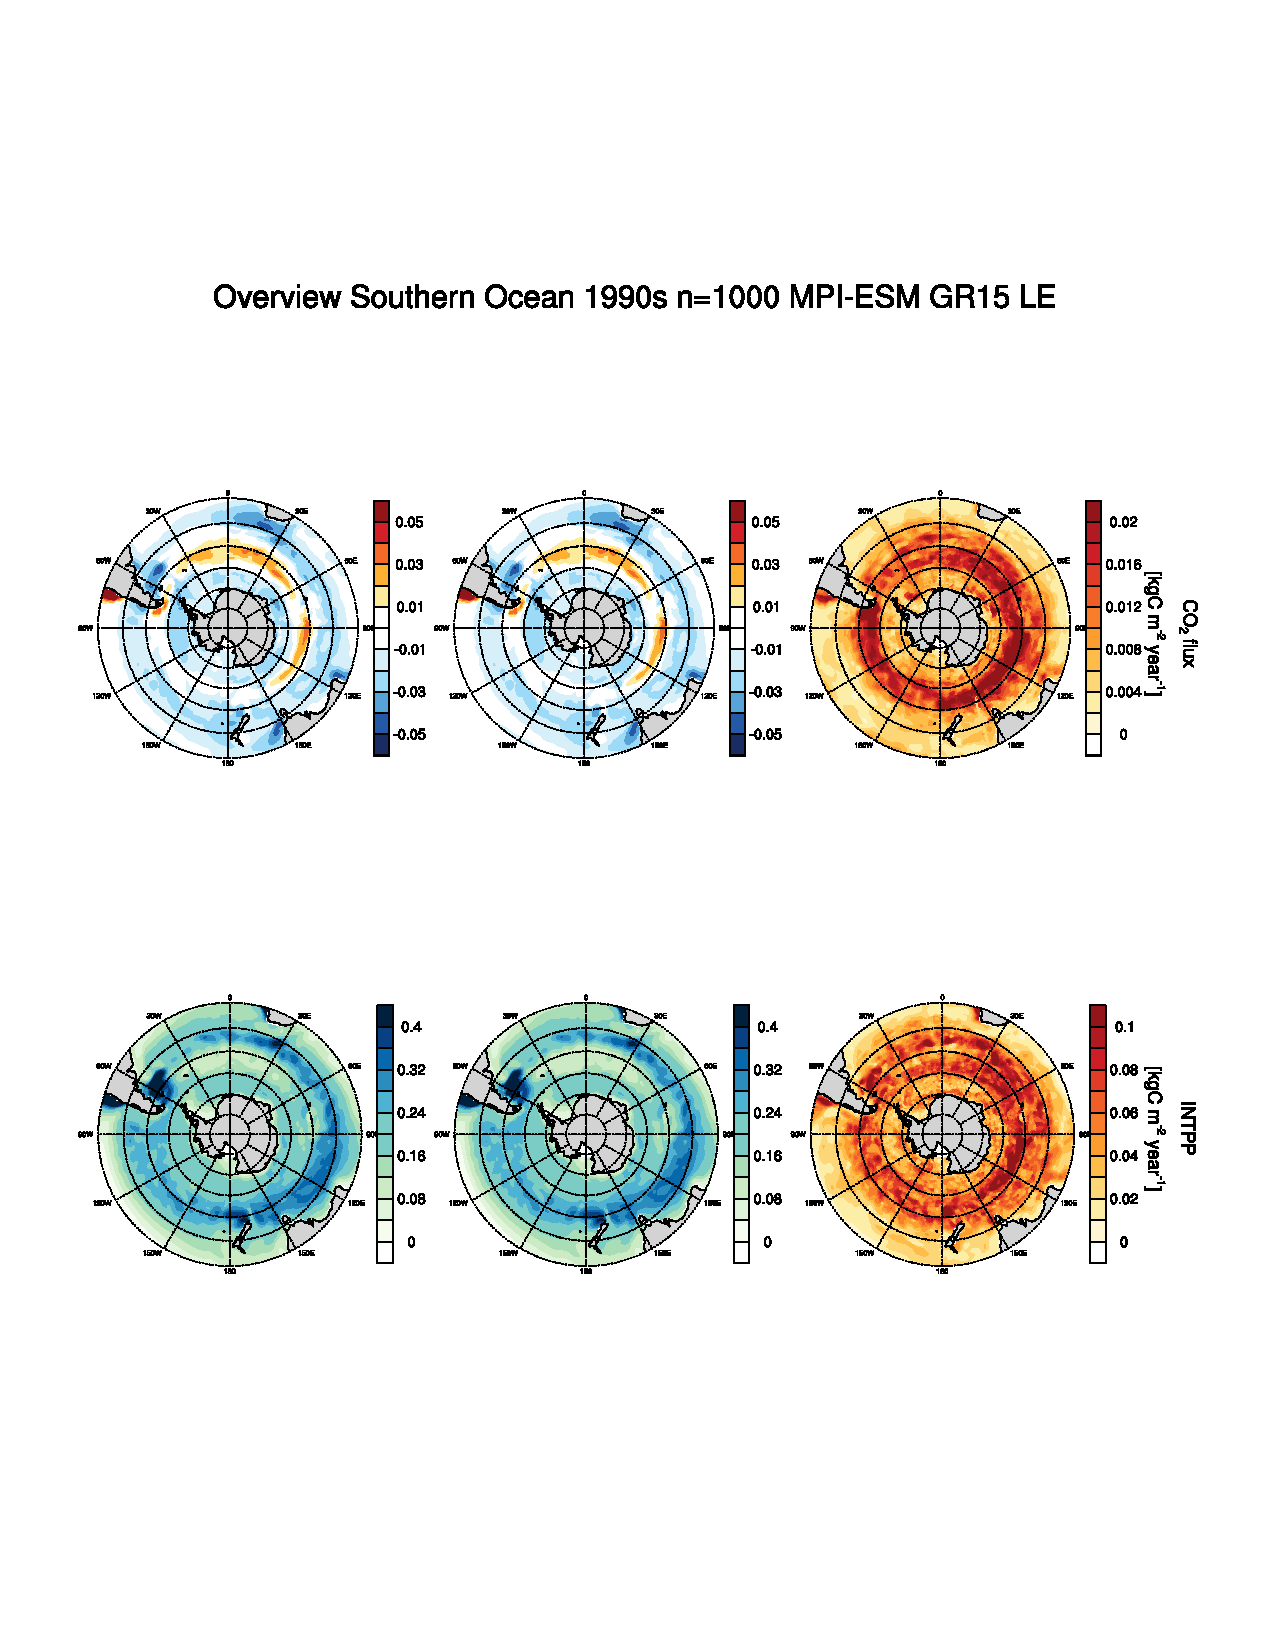
\includegraphics[scale=1.,page=1,trim=7.2cm 15cm 0cm 8cm,clip]{Overview_SO_co2flux_intpp_ens_t1990s.pdf} % co2flux
	\includegraphics[scale=1.,page=2,trim=7.2cm 15cm 0cm 8cm,clip]{Overview_SO_co2flux_intpp_ens_t1990s.pdf} % co2flux Landschuetzer
	\caption{Spatial distribution of the climatology (a,c) and decadal internal variability $\sigma_{DIV}$ (b,d) from 1980-2004 of the Southern Ocean air-sea CO$_2$ flux: MPI-ESM LE ensemble mean as forced signal (a), ensemble decadal standard deviation as decadal internal variability $\sigma_{DIV}$ (b), SOM-FFN climatology 1982-2004 (c), SOM-FFN decadal variability $\sigma_{DIV}$ (d); negative values indicate ocean uptake.}
	\label{fig:SOCS_ensmean_ensstd}
\end{figure}


\paragraph{Temporal evolution of the mean state and internal variability}
The modeled temporal evolution of the Southern Ocean ensemble mean CO$_2$ flux south of 35$^\circ$S is dominated by the forced negative trend of rising atmospheric CO$_2$ concentrations (fig. \ref{fig:evolution_southern_ocean_carbon_sink}). However, no individual realization follows the negative trend strictly monotonic - they oscillate around the ensemble mean state triggered by internal variability. Exemplary, the most extreme monotonic positive and negative 8-year trend is highlighted. Modeled decadal internal variability $\sigma_{DIV}$ is 0.22 PgC. 



\paragraph{Temporal comparison to observational data} 
The observational-based estimate for the whole region south of 35$^\circ$S shows a strong positive CO$_2$ flux trend in the 1990s \citep{LeQuere2007} and a strong negative CO$_2$ flux trend, reinvorgating the carbon sink in the 2000s  \citep{landschuetzer2015} (fig. \ref{fig:evolution_southern_ocean_carbon_sink}). 
The modeled $\sigma_{DIV}$ is lower than of the decadal variations of SOM-FFN. The decadal variability $\sigma_{DIV}$ in SOM-FFN data is 0.35 PgC, with the most positive CO$_2$ flux trend in the 1990s of $+0.40$ PgC and the most negative trend  of $-0.72$ PgC. These values of $\sigma_{DIV}$ suggest that these magnitudes in trends could be due to internal variability with a probability of 5\% ($\sim2\sigma$) and $0.2$\% ($\textgreater3\sigma$) for 1990s and 2000s trends respectively. This outlines how unlikely these observed CO$_2$ flux trends can be attributed to internal variability from the perspective of numerical modeling.   

The modeled internal variability of an interactive carbon cycle would be a more realistic counterpart for the observed internal variability, as the MPI-ESM LE simulations are forced with prescribed atmospheric CO$_2$ concentrations. The internal variability with an interactive carbon cycle produces 25\% higher internal variability because of the non-linear changes in atmoshperic CO$_2$ concentrations due to terrestrial carbon uptake \citep{Ilyina2013}.


\begin{figure}%[h!]
	\includegraphics[scale=.55,angle=90,page=2,trim=4cm 0cm 4cm 0cm,clip]{co2flux_SO_timeseries_ymjm_35S_1980_2015_trend_8}
	\caption{Temporal evolution of the Southern Ocean air-sea CO$_2$ flux south of 35$^\circ$S. Grey lines show the 100 ensemble members, the black line the ensemble mean, the blue shading is the ensemble decadal internal variability $\sigma_{DIV}$, the red line shows a positive CO$_2$ flux trend, the blue line shows a negative CO$_2$ flux trend, the green line represents the SOM-FFN observation-based estimate \citep{landschuetzer2015}; negative values indicate carbon uptake}
	\label{fig:evolution_southern_ocean_carbon_sink}
\end{figure}

%\paragraph{Choice of trends} 
%To analyze the processes driving this decadal internal variability $\sigma_{DIV}$, I focus on individual ensemble realizations. Here, I have to make a compromise between signal strength and robustness versus trendlength. It is a trade-off between decadal and inter-annual variability. The longer a period, the more likely the trend deviates from a monotonic behavior. Therefore longer trends show a less strong signal per trendlength (Fig. \ref{fig:heatmap}). Longer trends also experience a stronger influence of atmospheric forced trend. I decided to analyze 8-year trends, because they are still very close to a decade, but still they are able to show similar magnitude and monotonic behavior as the observation-based estimate. 


\paragraph{Highlighted monotonic CO$_2$ flux trends}
I select the most extreme positive and negative monotonic trends. 
Applying this selection criteria, I highlight two extreme CO$_2$ flux trends in fig. \ref{fig:evolution_southern_ocean_carbon_sink}. Analyzing a range of trendlengths from 6 to 14 years, I assess that MPI-ESM LE is able to capture positive and negative multi-year and decadal CO$_2$ flux trends in the Southern Ocean (Fig. \ref{fig:heatmap}). For decadal 10-year trends, the most extreme cases are of the same magnitude as those observed in the 1990s and 2000s  \citep{LeQuere2007,landschuetzer2015} (Fig. \ref{fig:heatmap}). 

I choose extreme monotonic trends to study the processes driving internal variability in the carbon cycle because stronger trends will give me a stronger signal in the underlying processes, which are discussed in chapter \ref{ch:trends}. %Therefore, I choose to analyze 8-year trends which are a compromise between trendlength (supposed to be 10 year for decadal variability) and a clearer signal (decays over time).

%The positive CO$_2$ flux trend highlighted in red is 0.7 PgC/8yrs, the negative CO$_2$ flux trend highlighted in blue is -0.8 PgC/8yrs. Those trends are higher than the corresponding trends in the 1990s and 2000s from SOM-FFN, but they that's also not the point of my study.  


\paragraph{Comparison of ensemble CO$_2$ flux internal variability} This is in contrast to other perturbed inital conditions large ensembles (see section \ref{sec:PICLE}). Neither CESM LE nor GFDL LE can reproduce similar strong decadal CO$_2$ flux trends in the Southern Ocean [personal communication Nikki Lovenduski, Sarah Schlunegger]. \cite{McKinley2016} mentioned a weak carbon sink for CESM LE. \cite{Resplandy2015} showed that MPI-ESM's dominant area of internal variability is the Southern Ocean, whereas CESM is most variable in the tropical and indian pacific and GFDL LE has large internal variability in tropical indian pacific as well as the Southern Ocean.

The different method of initialization could not have caused the behavior of trends, because the C0$_2$ flux pathways of different realizations already cross after few years and upper ocean loses his history after 50 years. The internal variability specific to the model itself is dominating \citep{Lovenduski2016}.  







\clearpage
\subsection{Winds}
\label{sec:winds_model_eval}
\paragraph{Spatial distribution in the mean state}
%The Southern Ocean is located on the Southern hemisphere around the Antarctic continent. As the atmospheric waves are disturbed by only few land masses and the insolation changes latitudinal, the Southern ocean carries very zonally symmetric features.
Winds are governed by distributions in sea-level pressure. They point from high pressure to low pressure systems, but get diverted to their left in the Southern hemisphere by the Coriolis force. Therefore, strong westerly winds are established between the low-pressure system south of 45$^\circ$S and higher pressure systems over the subtropical gyres (fig. \ref{fig:SO_winds_ensmean_ensstd}a). This is zonally symmetric SLP pattern in the ensemble climatological mean leads to zonally symmetric westerly winds peaking at 50$^\circ$S and decaying further northwards.

\paragraph{Spatial mean comparison to observational data}
The spatial zonal distribution in observational data from a NCEP reanalysis climatology is so similar to the MPI-ESM LE climatology that I plot the difference between MPI-ESM LE climatology and NCEP reanalysis \citep{Kalnay1996} (fig. \ref{fig:SO_winds_ensmean_ensstd}c). The position of the jets in ECHAM is shifted to lower latitudes \citep{Stevens2013} which seems to be a common atmospheric modeling challenge \citep{Kidston2010}. Therefore, the modeled westerlies are too strong from 30-60$^\circ$S and too weak south of 60$^\circ$S. The zonal wind speed difference peaks at 45$^\circ$S at +1m/s. 

\paragraph{Spatial distribution of internal variability} 
The decadal internal variability $\sigma_{DIV}$ increases zonally towards lower latitudes with the highest internal decadal variability in the pacific sector in the Southern Ocean seasonal ice-covered area (fig. \ref{fig:SO_winds_ensmean_ensstd}b).

\paragraph{Spatial internal variability comparison to observational data}
Observational reanalysis data reveal the same spatial distribution with a higher amplitude of decadal internal variability (fig. \ref{fig:SO_winds_ensmean_ensstd}d). The pacific sector reflects the area of an Antarctic dipole induced from the El N\~{n}o-Southern Oscillation (ENSO), which manifests itself in variability of sea-ice \citep{Yuan2004}. This is also known as the Pacific-South American (PSA) Oscillation \citep{Sallee2008}. The atmospheric Southern Ocean jet splits and in El Ni\~{n}o conditions intensifies on a northern route which induces a low pressure system with more storms. La Ni\~{n}a conditions bring a high pressure system with less storms vice versa. Such tele-connections of the tropics into the Southern Ocean are subject of current research and rarely analyzed for the Southern Ocean carbon sink.  

%The direction of winds is lost in the calculation of standard deviations, therefore the wind arrows in fig. \ref{fig:SO_winds_ensmean_ensstd}b,d only show the magnitude of the internal variability of winds which is highest in the pacific sector of the Southern Ocean and generally decreases with latitude.

\begin{figure}[h!]
	\centering
%	\llap{ \parbox[b]{0cm}{\textbf{a}\\\rule{0ex}{0cm}}}
%	\hspace{3cm} \llap{ \parbox[b]{2cm}{\textbf{b}\\\rule{0ex}{0cm}}}
	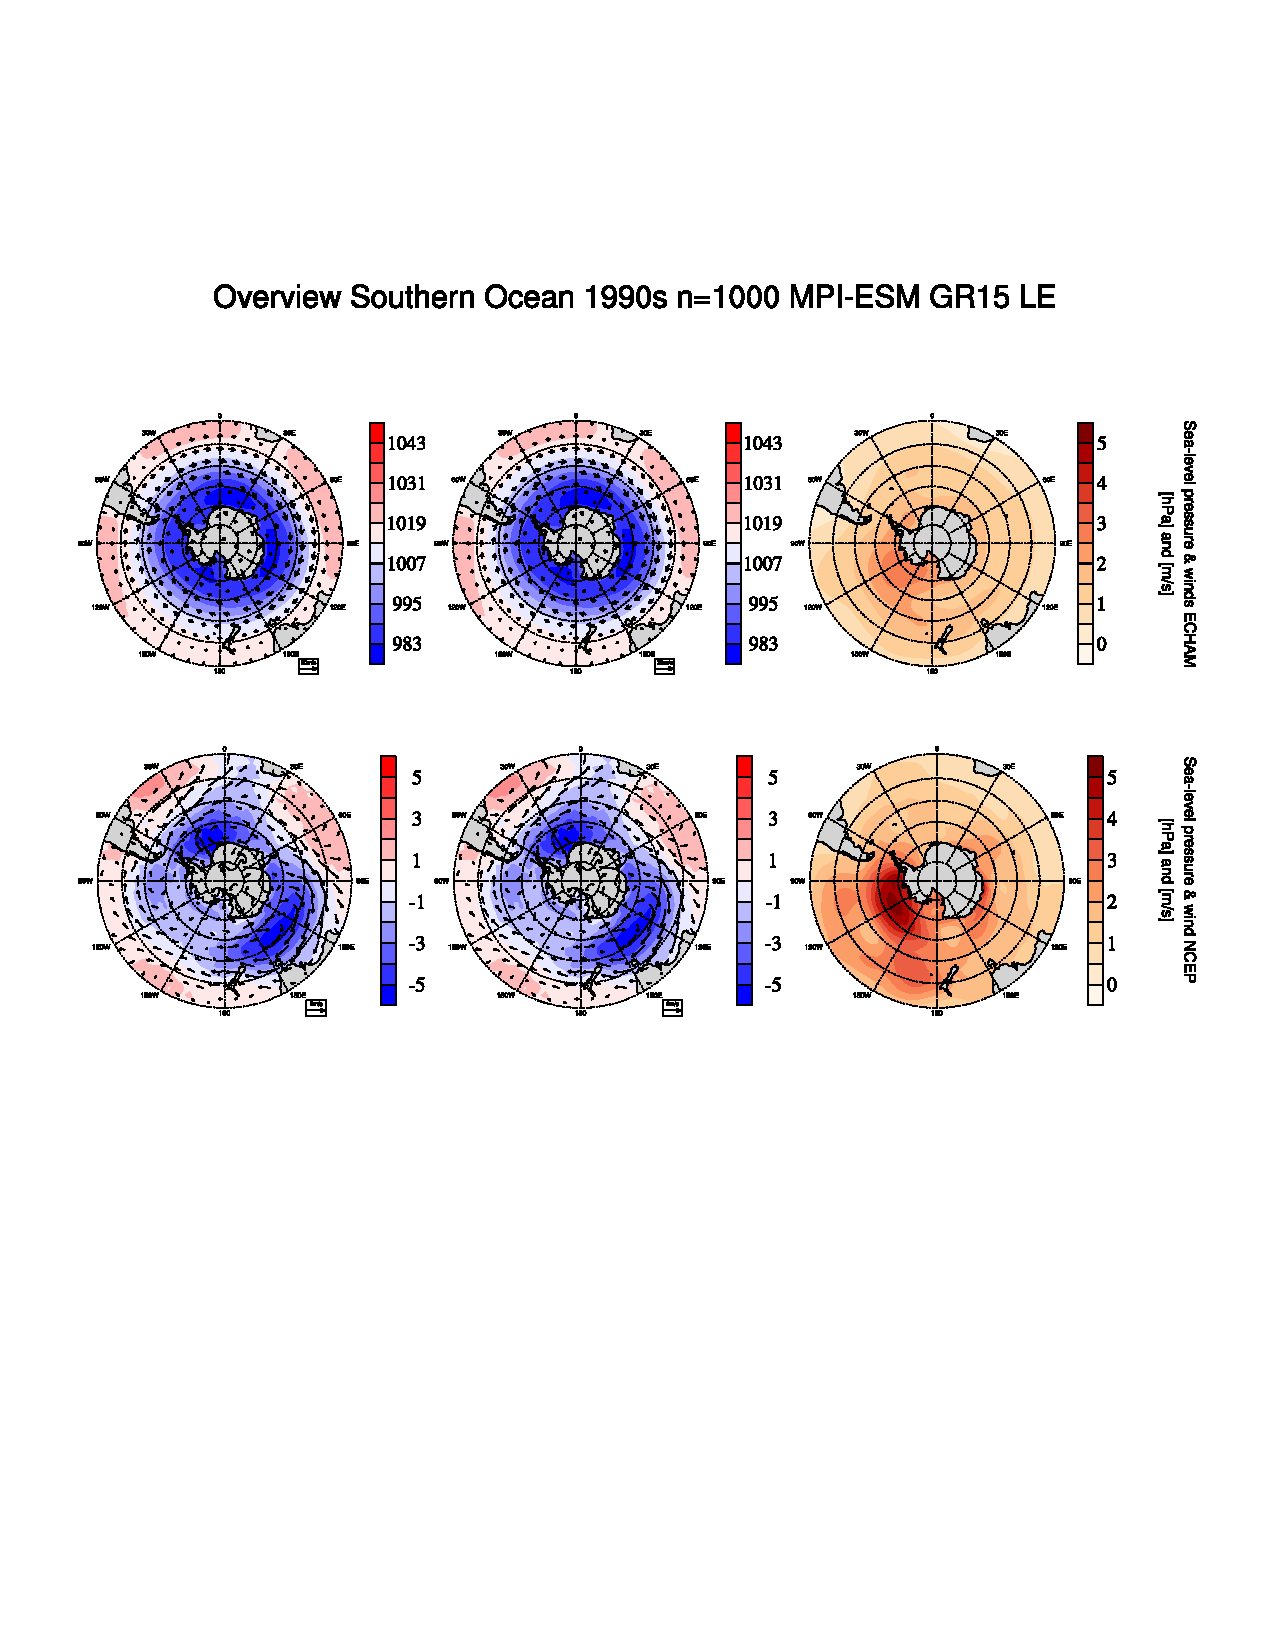
\includegraphics[scale=1.,trim=7.3cm 16.2cm 0cm 6.9cm,clip]{Overview_SO_slp_ens_t1990s.pdf} % echam
	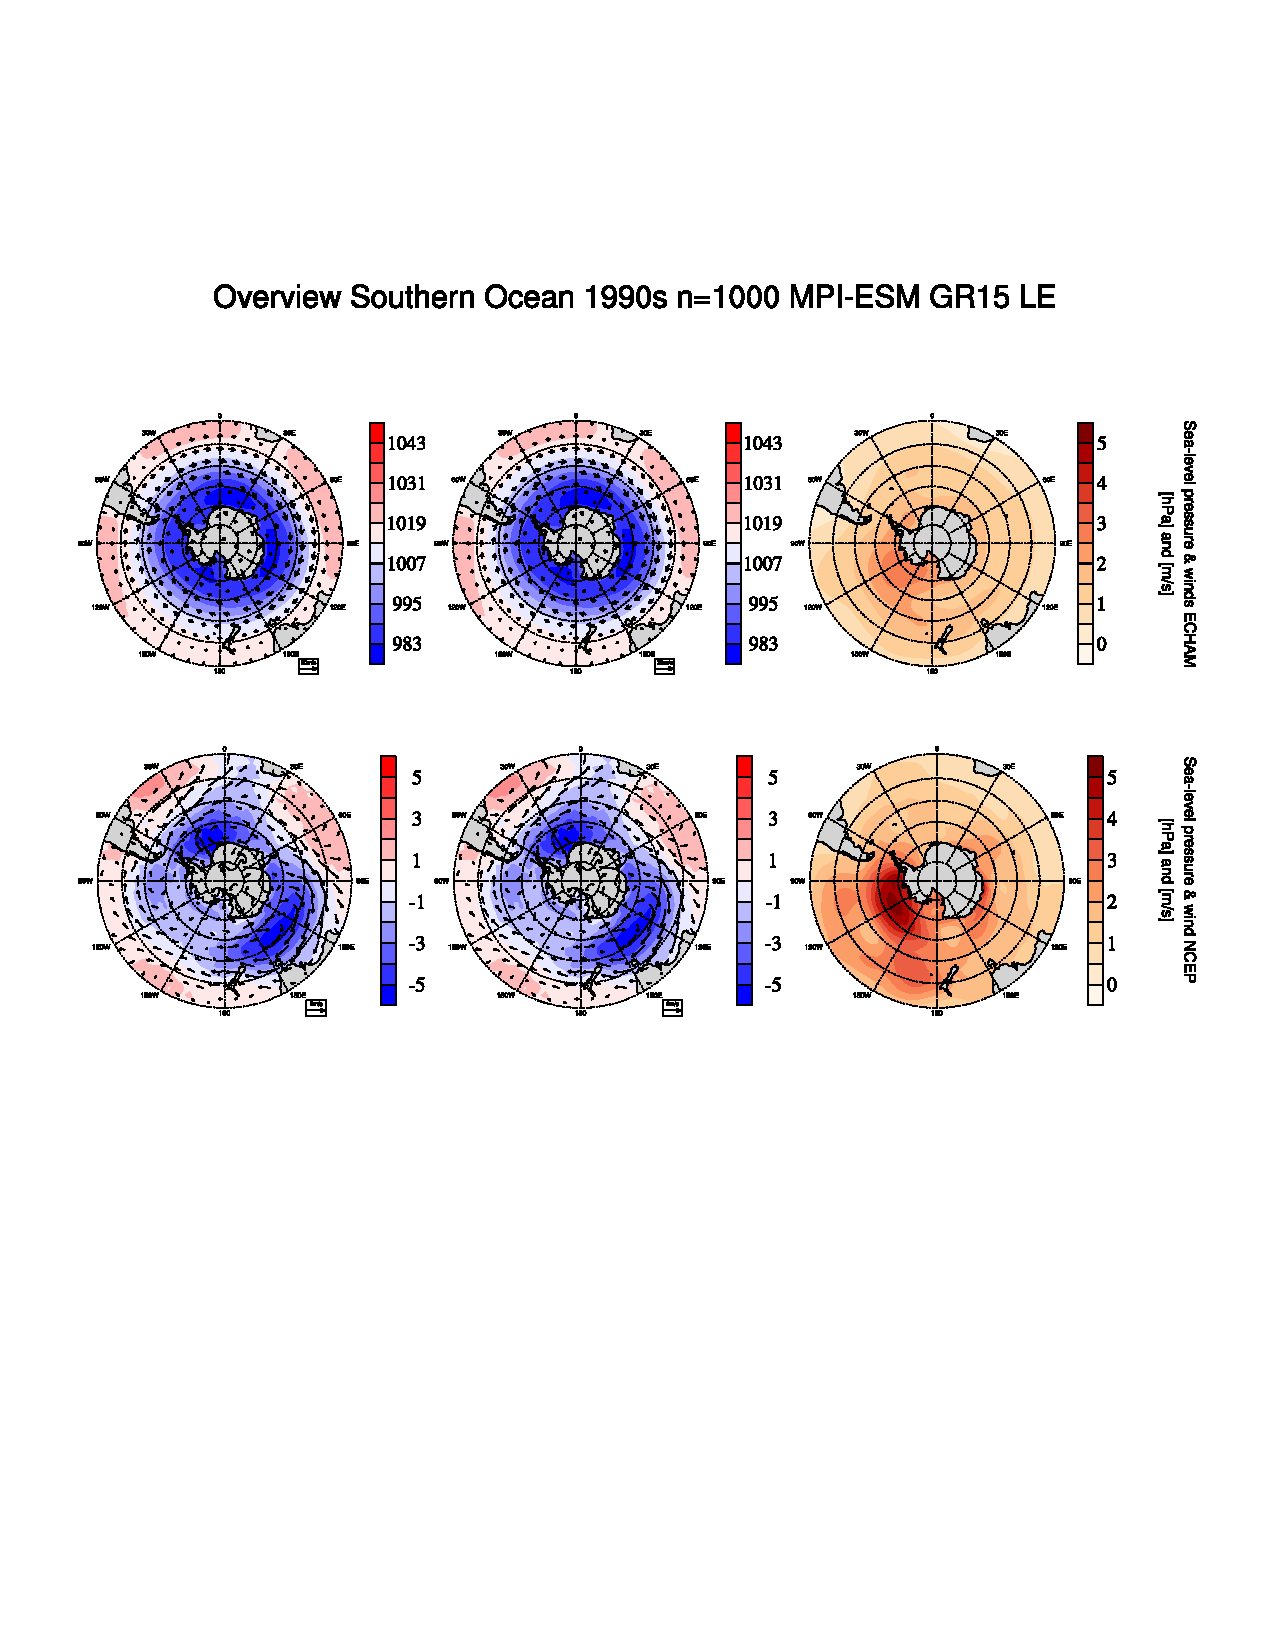
\includegraphics[scale=1.,trim=7.3cm 10.6cm 0cm 12.5cm,clip]{Overview_SO_slp_ens_t1990s.pdf} % ncep
	\caption{Spatial distribution of the Southern Ocean sea-level pressure and wind vectors overlain as arrows: ensemble mean climatology from 1980 to 2004 (a) as forced signal and ensemble decadal standard deviation (b) as decadal internal variability $\sigma_{DIV}$; and the difference between MPI-ESM and reanalysis data from NCEP climatology \citep{Kalnay1996} (c), and decadal internal variability $\sigma_{DIV}$ from NCEP climatology (d).}
	\label{fig:SO_winds_ensmean_ensstd}
\end{figure}

\paragraph{Temporal evolution of the mean state and internal variability}
Fig. \ref{fig:SO_winds_ensmean_ensstd} shows the temporal evolution and internal variability of the annual Southern Annular Mode (SAM) index calculated according to \citep{Gong1999} (see section \ref{sec:sam}). Positive SAM index values are associated with anomalously a low sea-level pressure over Antarctica which result in a southward shift and intensification of westerly winds. The ensemble mean has a positive trend. This trend is a consequence to anthropogenic CO$_2$ emission and ozone depletion over Antarctica \citep{Thompson2000}.

\paragraph{Temporal comparison to observational data} 
MPI-ESM LE SAM index lies in the range of the station-based from \citep{Marshall2003}, although it follows a weaker trend in the ensemble mean. 

\paragraph{Temporal evolution of extreme carbon trend members}
The positive CO$_2$ flux trend shows a positive trend in SAM. Those strengthening winds increase upwelling (see section \ref{sec:UOOC}), which brings waters over-saturated in DIC to the surface and hence lead to outgassing anomalies. This weakens the carbon sink and vice versa strengthens the carbon sink under the context of weakening westerly winds. The detailed response of primary production and upwelling under the context of changing winds is discussed in chapter \ref{ch:trends}.







\begin{figure}[h!]
	\includegraphics[scale=.55,angle=90,trim=4cm 0cm 4cm 0cm,clip,page=4]{co2flux_SO_timeseries_ymjm_35S_1980_2015_trend_8}
	\caption{Temporal evolution of the annual Southern Annular Mode (SAM) index according to \citep{Gong1999}. Grey lines show the 100 ensemble members; the black line the ensemble mean; the blue shading is the decadal internal variability $\sigma_{DIV}$; the red line reprensents positive CO$_2$ flux trend; the blue line shows the negative CO$_2$ flux trend; the green line shows the station-based SAM from \cite{Marshall2003}}
	\label{fig:evolution_SAM}
\end{figure}






\clearpage
\subsection{Biology}
\label{sec:biology}

\paragraph{Spatial distribution in the mean state} %going from coast to north
(fig. \ref{fig:SOCS_ensmean_ensstd}a) 
The strong seasonal cycle in insulation and the spraseness of land topography leads to first-order zonally symmetric constraints for light and sea-surface temperature (SST). The high-latitude Southern Ocean is a so-called high nutrient low chlorophyll (HNLC) region, where light is the dominant limiting factor for the low biological production, but nutrients are plenty \citep{Falkowski1998}. Summer sea-ice cover and sub-zero SST values constrain plankton growth and is responsible for the tiny amount of primary production in the coastal areas as well as the Ross Sea and Weddell Sea. 

With decreasing latitude in the Southern Ocean, primary production increases along with increasing temperatures and light availability. Nutrients are upwelled by the upper-ocean overturning circulation and advected northwards by Ekman transport. This latitudinal increase of primary production peaks at 40-50$^\circ$S, where nutrients are abundant from upwelling and Ekman transport and higher temperatures and light availability foster phytoplankton growth rates. The mixing with warm subtropical waters off the Argentinian coast increases SST and leads to a maximum primary production in the Southern Ocean \citep{Behrenfeld2014}. Downstream the Drake passage, the polar front with its cold waters extends more northward \citep{Orsi1995}. Along with lower nutrient concentrations due to increased precipitation from storms explains the relatively low primary production in the Atlantic sector compared to other longitudinal counterparts. 

At the subtropical front, decreasing nutrient concentrations limit primary production \citep{Behrenfeld2014}. 


\paragraph{Spatial mean comparison to observational data}
To evaluate HAMOCC's ability to model the Southern Ocean, I do not compare modeled primary production to chlorophyll-a  concentration derived from satellite data, because satellite images are frequently  hidden by clouds. Instead, I compare the distributions of nitrate which is the limiting nutrient for biological production in this HAMOCC version. %nitrate would be the limiting one
The distribution of nitrate shows a strong gradient in HAMOCC as well as in the  World Ocean Atlas (WOA) 2013  \citep{WOA2013} along the fronts from low-nutrients in the high-latitudes to nutrient depletion in the subtropical gyres (fig. \ref{fig:SO_comp_nitrate}). In higher latitudes HAMOCC underestimates the phosphate concentration by 25\%. These lower nutrient concentrations can be a sign of more nutrient consumption at higher primary production or be the reason for lower primary production. The distribution of another important nutrient phosphate shows a similar spatial pattern (fig. \ref{fig:SO_comp_phosph}).

\paragraph{Spatial distribution of internal variability} 
Internal decadal variability in vertically integrated primary production in the Southern Ocean is higher in high productivity areas (fig. \ref{fig:SO_intpp_ensmean_ensstd}b). The whole region at 45-60$^\circ$S, especially in the Indian sector, shows a enormously high decadal internal variability $\sigma_{DIV}$ relative to the ensemble mean state. Internal variability in the Southern hemisphere is mostly driven by westerly winds. The explicit effect of those on HAMOCC is discussed in chapter \ref{ch:trends}. 

\begin{figure}[h!]
	\centering
	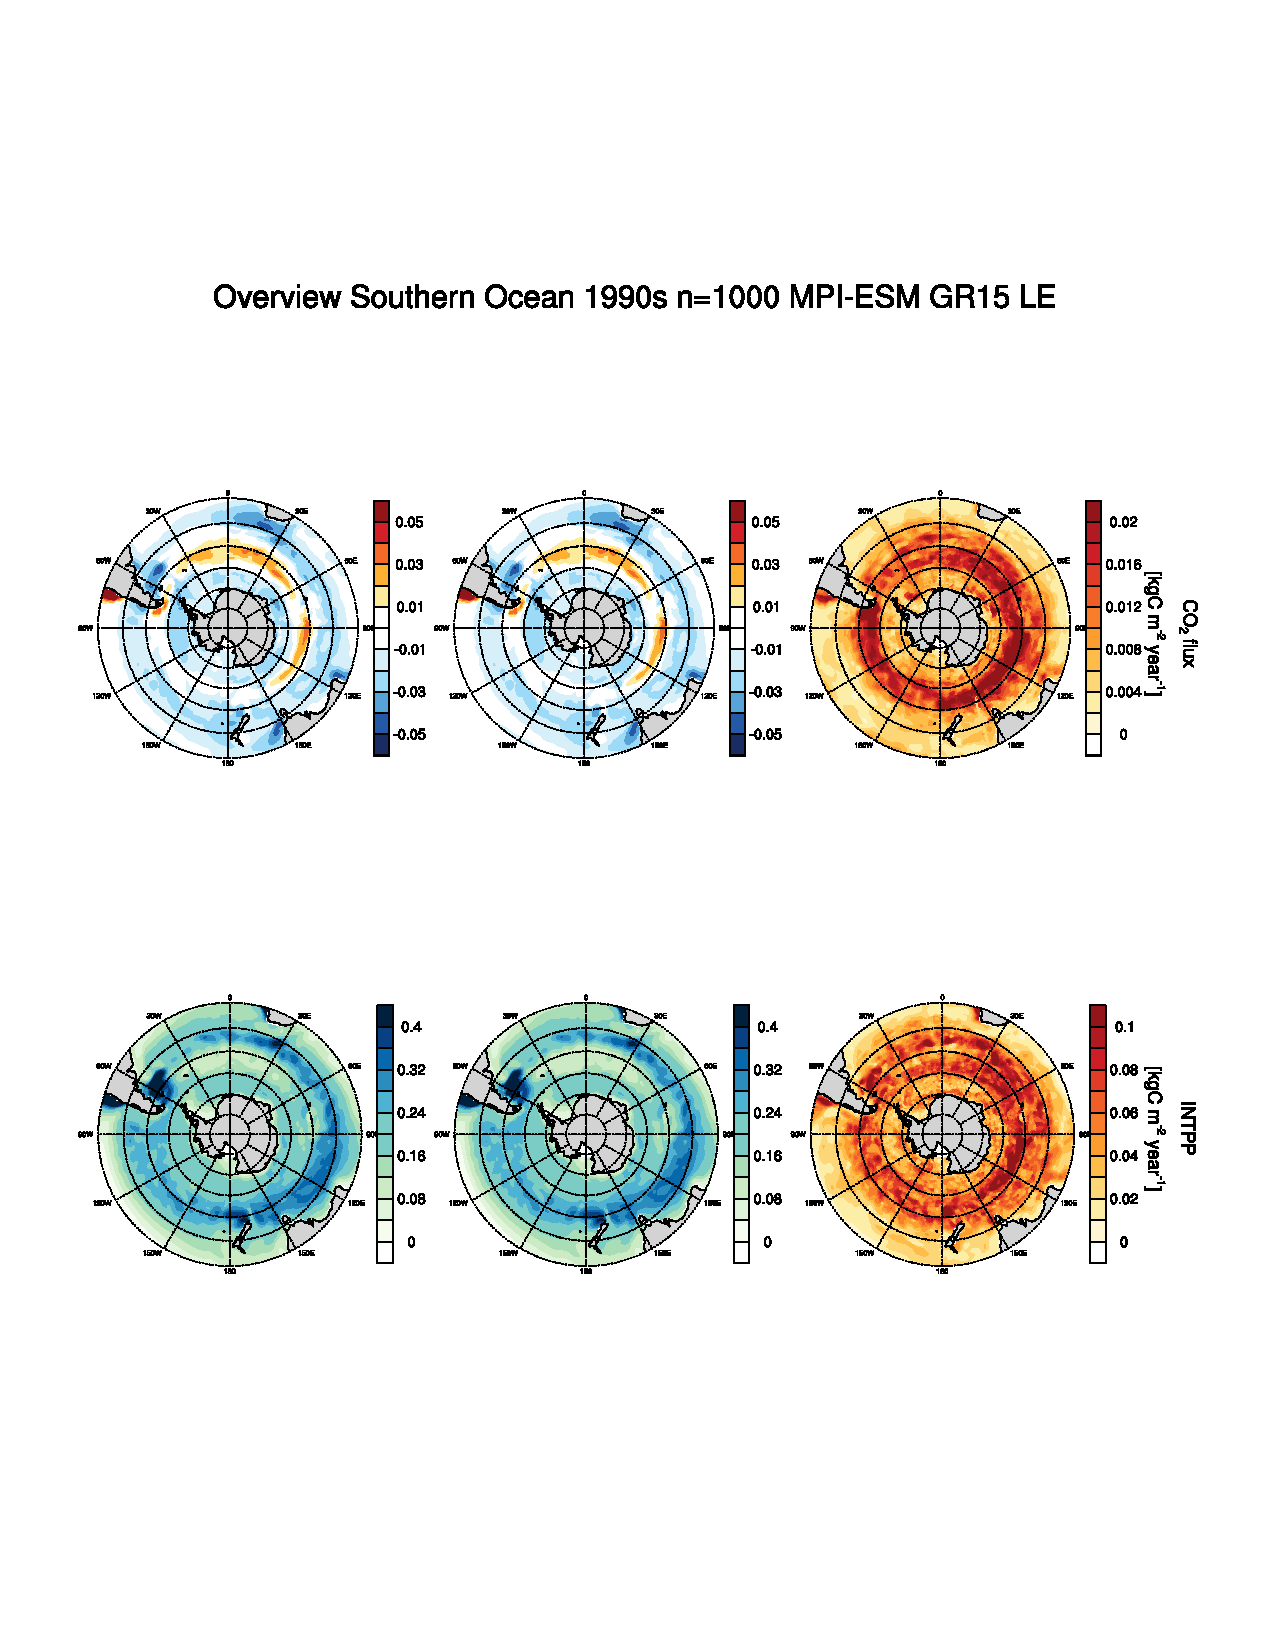
\includegraphics[scale=1.2,trim=7.2cm 6.3cm 0cm 16cm,clip]{Overview_SO_co2flux_intpp_ens_t1990s.pdf} % intpp
	\caption{Spatial distribution of the vertically integrated primary production in the Southern Ocean: climatological ensemble mean from 1980 to 2004 (left) as forced signal and ensemble decadal anomaly standard deviation (right) as decadal internal variability $\sigma_{DIV}$}
	\label{fig:SO_intpp_ensmean_ensstd}
\end{figure}

\begin{figure}[h!]
	\centering
	\includegraphics[scale=.85,page=3,trim=1.8cm 13.3cm .8cm 6.5cm,clip]{Overview_SO_nutrient_comparison.pdf} % nitrate
	\caption{Spatial distribution of the climatology of surface nitrate (left) compared with WOA data \citep{WOA2013} (right)}
	\label{fig:SO_comp_nitrate}
\end{figure}



\paragraph{Temporal evolution of the mean state and internal variability}
Primary production in the Southern Ocean is not subject to a strong forced trend in the historical period, but varies internally (fig. \ref{fig:evolution_southern_ocean_intpp}). The weak decreasing trend might be the first signs of increased stratification due to sea-surface warming, which in turn inhibits the mixing of nutrients. But the long-term consequences for primary production is subject to ongoing research and debate \citep{Bopp2013,Taucher2011,Lozier2011,Kessler2016,Krumhardt2017}. The decadal internal variability $\sigma_{DIV}$ is 0.5 PgC.

The absolute amount of primary production exceeds CO$_2$ flux by a factor of $\sim$20. The spatial distribution of export flux at 90m, which is the particulate organic matter that sinks below the euphotic zone before being remineralzed, is the same as for primary production. As a lower vertical boundary for a upper-ocean carbon budget of the euphotic zone, export flux is of similar magnitude as CO$_2$ flux and thus comparable, see chapter \ref{ch:pCO2separation}.

\paragraph{Temporal evolution of extreme CO$_2$ flux trends}
The negative CO$_2$ flux trend has a positive trend in primary production, because primary production lowers surface DIC, pCO$_{2\text{,ocean}}$ and hence reduces CO$_2$ uptake by the ocean; and vice versa negative trends in primary production lead to positive CO$_2$ flux trends.

\paragraph{HAMOCC Southern Ocean performance}
MPI-ESM is able to model the general features of the Southern Ocean, such as the characteristics of a high nutrient low chlorophyll region \citep{Bopp2013}. But compared to other models and observational data, the seasonal cycle of phytoplankton blooms is amplified and too early in the Southern Ocean \citep{Bopp2013,Nevison2016}. The reason of this is under current debate in the MPI biogeochemistry research group. It could involve that the Southern Ocean in MPI-ESM LE run is not iron-limited. Furthermore, the atmospheric bias in westerly winds and the Southern Ocean warm bias \citep{Jungclaus2013} hinders sea-ice to propagate more extensively. A proper representation of Antarctic sea-ice would come along with a cooler, more stratified Southern Ocean which modulates primary production.

Additionally, the longest standing data records, which are on the northern hemisphere in Iceland \citep{Six1996}, are used for the tuning of free model parameters. The Southern Ocean has never been in the focus of HAMOCC. 






\begin{figure}[h!]
	\centering
	\includegraphics[scale=.6,angle=90,trim=4cm 0cm 4cm 0cm,clip,page=3]{co2flux_SO_timeseries_ymjm_35S_1980_2015_trend_8}
	\caption{Temporal evolution of the vertically integrated primary production in the Southern Ocean south of 35$^\circ$S. Grey lines show the 100 ensemble members, the black line the ensemble mean, the blue shading is the decadal internal variability $\sigma_{DIV}$, the red line reprensents the positive CO$_2$ flux trend, the blue line represents negative CO$_2$ flux trend}
	\label{fig:evolution_southern_ocean_intpp}
\end{figure}




\clearpage

\subsection{Upper-Ocean Overturning Circulation}
\label{sec:UOOC}

\paragraph{Spatial distribution in the mean state and internal variability}
The Southern Ocean upper-ocean overturning circulation is driven by the divergence at 40-60$^\circ$S corresponding to strong westerly winds. Fig. \ref{fig:UOOC_mean}a shows a zonal transect view of the ensemble mean circulation. 
The isopyncals, which separate water masses, orient themselves at values from \cite{Sallee2013a}, but are shifted to fit to typical depths, which is a common feature in water mass comparison as models have different density biases \citep{Sallee2013a}. 
In the high latitudes south of 50$^\circ$S, Ekman pumping brings Circumpolar Deep Water (CDW) from the ocean interior to the surface. At the surface, these waters are transported to the north. At lower latitudes, the surface waters warm and evaporation increases, so relatively cold and low salinity waters known as Antarctic Intermediate Water (AAIW) slide below warmer and more saline Subantarctic Mode Waters (SAMW) to extend northwards at intermediate depth. This process is called downwelling or Ekman subduction.  

The strong upper-ocean circulation features upwelling south of 50$^\circ$S, northward transport at 40-60$^\circ$S and downwelling at 30-40$^\circ$S and is known as the Deacon cell \citep{Doeoes1993,Speer2000}. The upper-ocean overturning circulation is driven by the strength and positions of westerly winds. Upwelling steepens and downwelling straightens the isopycnals along which the water masses flow. The internal variability in the horizontal processes at intermediate depth is lower than at the surface, because the influence of winds decays with depth. The decadal internal variability $\sigma_{DIV}$ of vertical Ekman pumping and subduction is of similar magnitude at 200m and 1000m (fig. \ref{fig:UOOC_mean}). 

\paragraph{Comparison to observational data}
Fig. \ref{fig:UOOC_mean}a is similar to Fig. 1 from \cite{DeVries2017} which uses observational data in an inverse model to demonstrate upper-ocean overturning circulation. Due to different vertical velocity regimes, I choose different boundaries for the transport, which prevents me from quantitative comparisons. Nevertheless, data of \cite{DeVries2017} Fig. 1 show the main characteristics of the Deacon cell and water transport of comparable magnitude as in MPI-ESM LE. 



\begin{figure}[h!]
	\centering
	%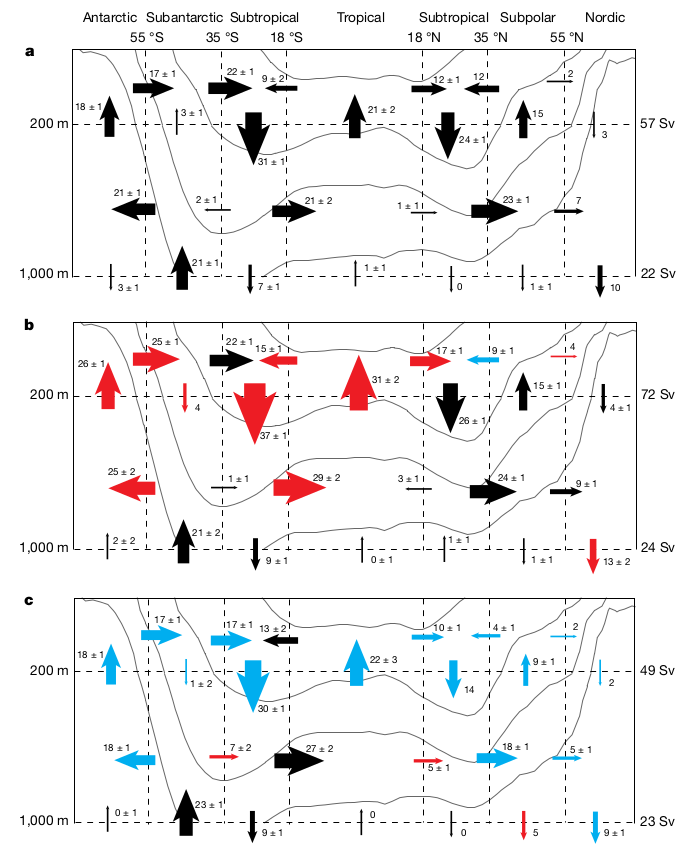
\includegraphics[scale=.7,trim=.3cm 14cm 0cm .6cm,clip]{DeVries_2017_Fig1_Upper_Ocean_Overturning_Circulation}	
	\llap{ \parbox[b]{0cm}{\textbf{a}\\\rule{3ex}{0cm}}} 
	\includegraphics[scale=0.5,page=4,trim=1.4cm 1.7cm 0cm 4.6cm,clip]{UOOC}
	\llap{ \parbox[b]{15cm}{\textbf{b}\\\rule{3ex}{0cm}}} 
%	\llap{ \parbox[b]{8.0cm}{\textbf{a}\\\rule{3ex}{3.7cm}}} 
	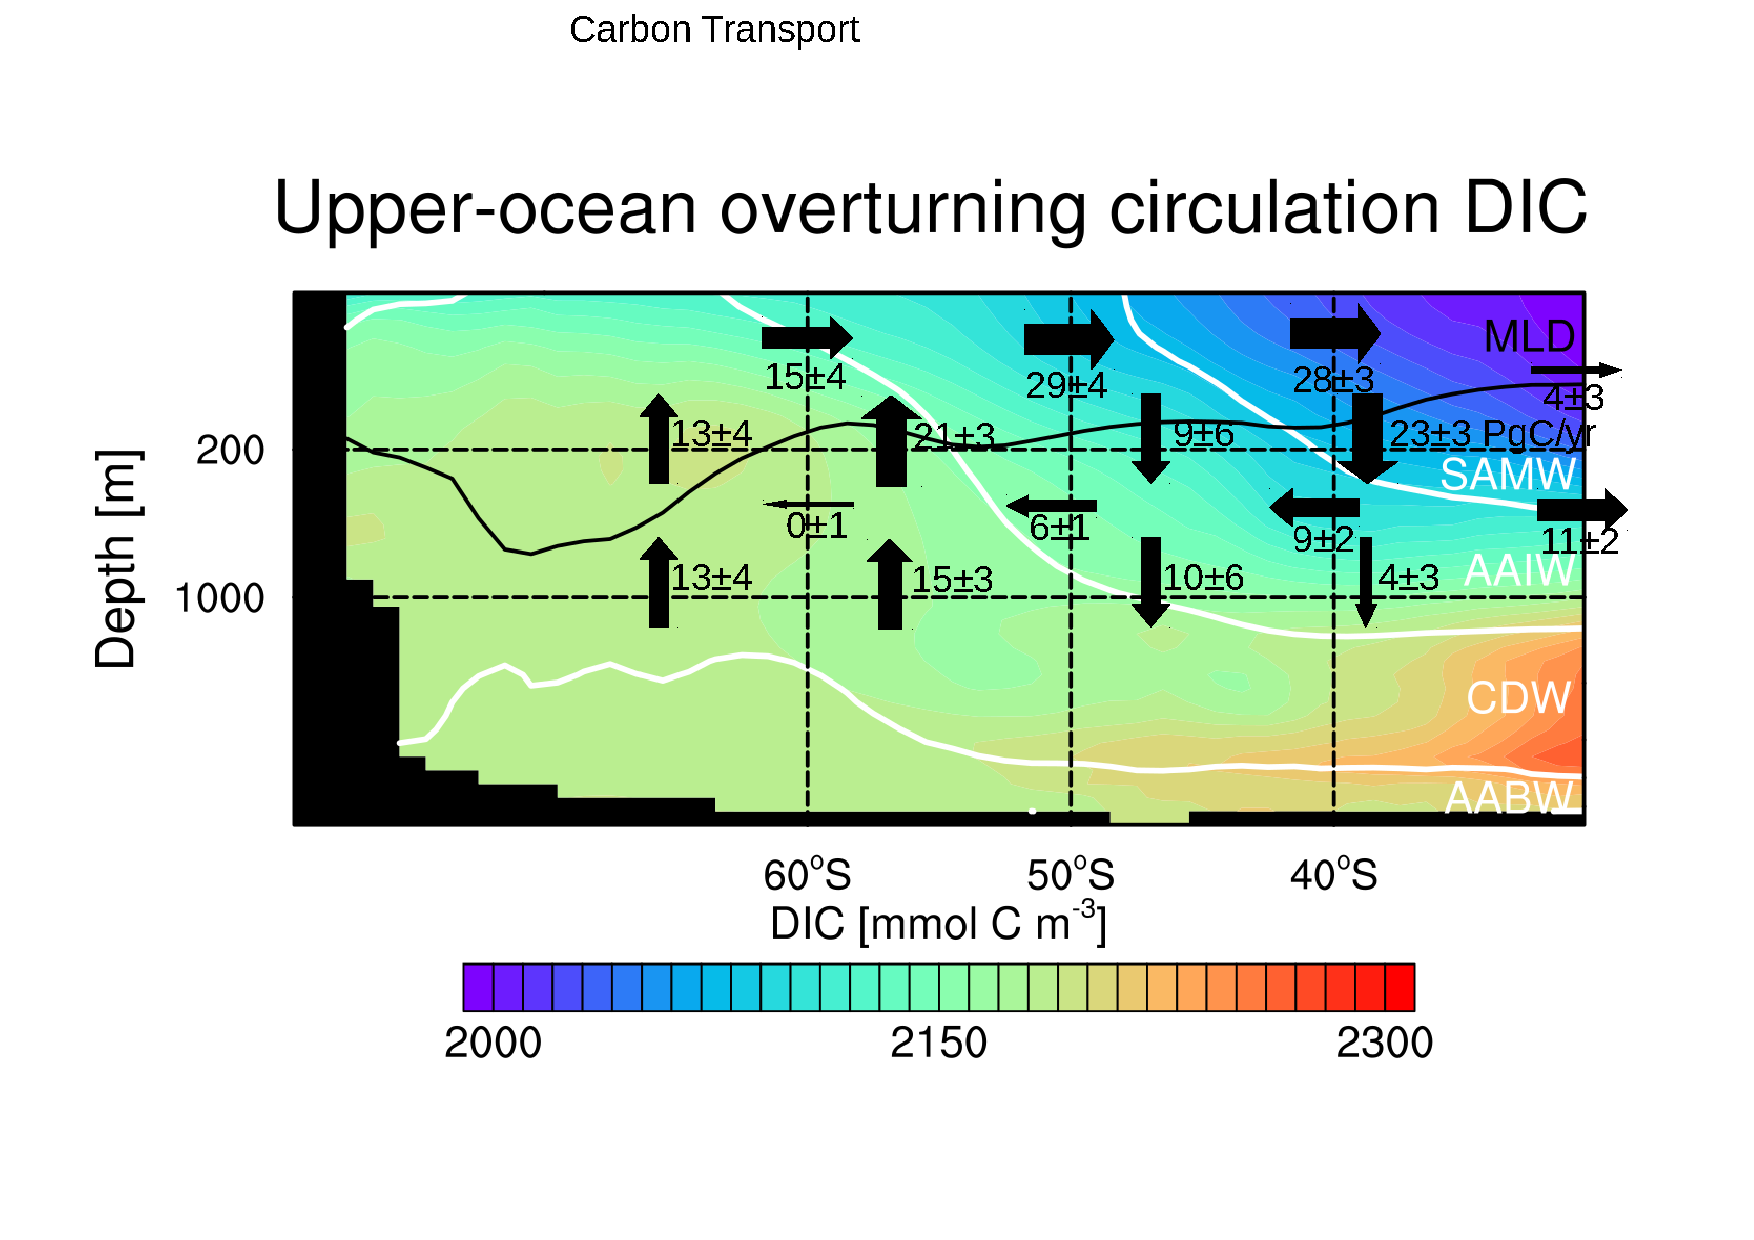
\includegraphics[scale=0.5,page=1,trim=1.4cm 1.7cm 0cm 4.6cm,clip]{UOOC}	
		%\llap{ \parbox[b]{8.0cm}{\textbf{a}\\\rule{0ex}{6.7cm}}} 
	\vspace{-8mm}
	\caption{Zonally averaged transect of the Southern Ocean and the upper-ocean overturning circulation; black arrows show yearly mean advective transports of water in Sv (a) and carbon in PgC/yr (b) and its decadal internal variability $\sigma_{DIV}$; white lines are isopyncals separating Sub-Antarctic Mode Water (SAMW) at potential density $\rho_{\theta\text{}}=1026.5$ kg m$^{-3}$ from Antarctic Intermediate Water (AAIW), at $\rho_{\theta\text{}}=1027.2$ kg m$^{-3}$ from Circumpolar Deep Water (CDW), at $\rho_{\theta\text{}}=1027.7$ kg m$^{-3}$ from Antarctic Bottom Water (AABW); the black line is the mixed-layer depth (MLD); the colored contours show the distribution of dissolved inorganic carbon (DIC)}
	\label{fig:UOOC_mean}
\end{figure}


\paragraph{Link to the carbon cycle}
The concentration of dissolve inorganic carbon (DIC) in general increases with depth due to the biological pump and remineralization at depth. This is most clearly seen in the subtropics and blurred by all processes of mixing at higher latitudes (fig. \ref{fig:UOOC_mean}). Still, upwelled waters from the deep oceans have a high pCO$_2$ potential at which they would equilibrate when lifted to the surface, so the upwelling super-saturated waters in high latitude waters drives CO$_2$ outgassing and downwelling takes CO$_2$ equilibrated waters into the deeper ocean (fig. \ref{fig:UOOC_mean}b). 

%\paragraph{Temporal evolution of the mean state and internal variability} I would need to construct an index

\paragraph{Trends of extreme carbon trend members}
The positive CO$_2$ flux trend shows intensified upper-ocean overturning circulation. This means enhanced upwelling, which weakens the carbon sink (Fig. \ref{fig:UOOC_neg}) and vice versa strengthen the carbon sink for weaker upper ocean overturning circulation (fig. \ref{fig:UOOC_pos}). %[I could to construct an index to have a similar figure as before, but dont know whether what would be really nessessary for the story.]

%\paragraph{Temporal comparison to observational data}  no data; a bit compared to DeVries


\paragraph{MPI-OM Southern Ocean performance evaluation}  
The global performance of MPIOM is discussed in detail in \cite{Jungclaus2013}. The Southern Ocean sea-surface temperature warm bias is attributed to an overestimation of downward shortwave radiation into the polar regions \citep{Stevens2013} and causes the underestimation of sea-ice coverage. Additionally, through open-ocean convection in the Ross and Weddel Sea and deeper than observed winter mixing, heat from the relatively warm circumpolar deep waters warm the subsurface waters \citep{Stoessel2015}. Additional freshwater input from melting glaciers distributed along the coast a basal meltwater and along the high-latitude Southern Ocean to mimic freshwater input due to icebergs would improve the water column stability to prevent open-ocean convection. The same effect would have the coupling to a higher resolved atmosphere due to additional freshwater input \citep{Stoessel2015}. 

%\subparagraph{Water mass circulation}
The model quality of overturning circulation in the Southern Ocean is analyzed by \cite{Sallee2013a}. MPI-ESM realistically simulates subtropical water temperature and SAMW in general. But the overturning cell is much weaker than in other models.

%\subparagraph{ZMLD comparison} 
The mixed-layer depth (MLD) is an important measure to assess how climate models represent the Southern Ocean. MLD in MPI-ESM is overestimated compared to observational data from NOAA Atlas \citep{Monterey1997}; spatially in the locations of the ACC and the Ross and Weddell Sea (fig. \ref{fig:SO_comp_zmld}) as well as in the zonal average (fig. \ref{fig:UOOC_mean}). In the Ross and Weddell Sea, the MLD deepens to few kilometers depth via open-ocean convection \citep{Stoessel2015}, which often appears in climate models but rarely seen in observations \citep{Heuze2013}. This and the weak stratification explains why MPI-ESM overestimates MLD in winter \citep{Sallee2013}.


\begin{figure}[h!]
	\centering
	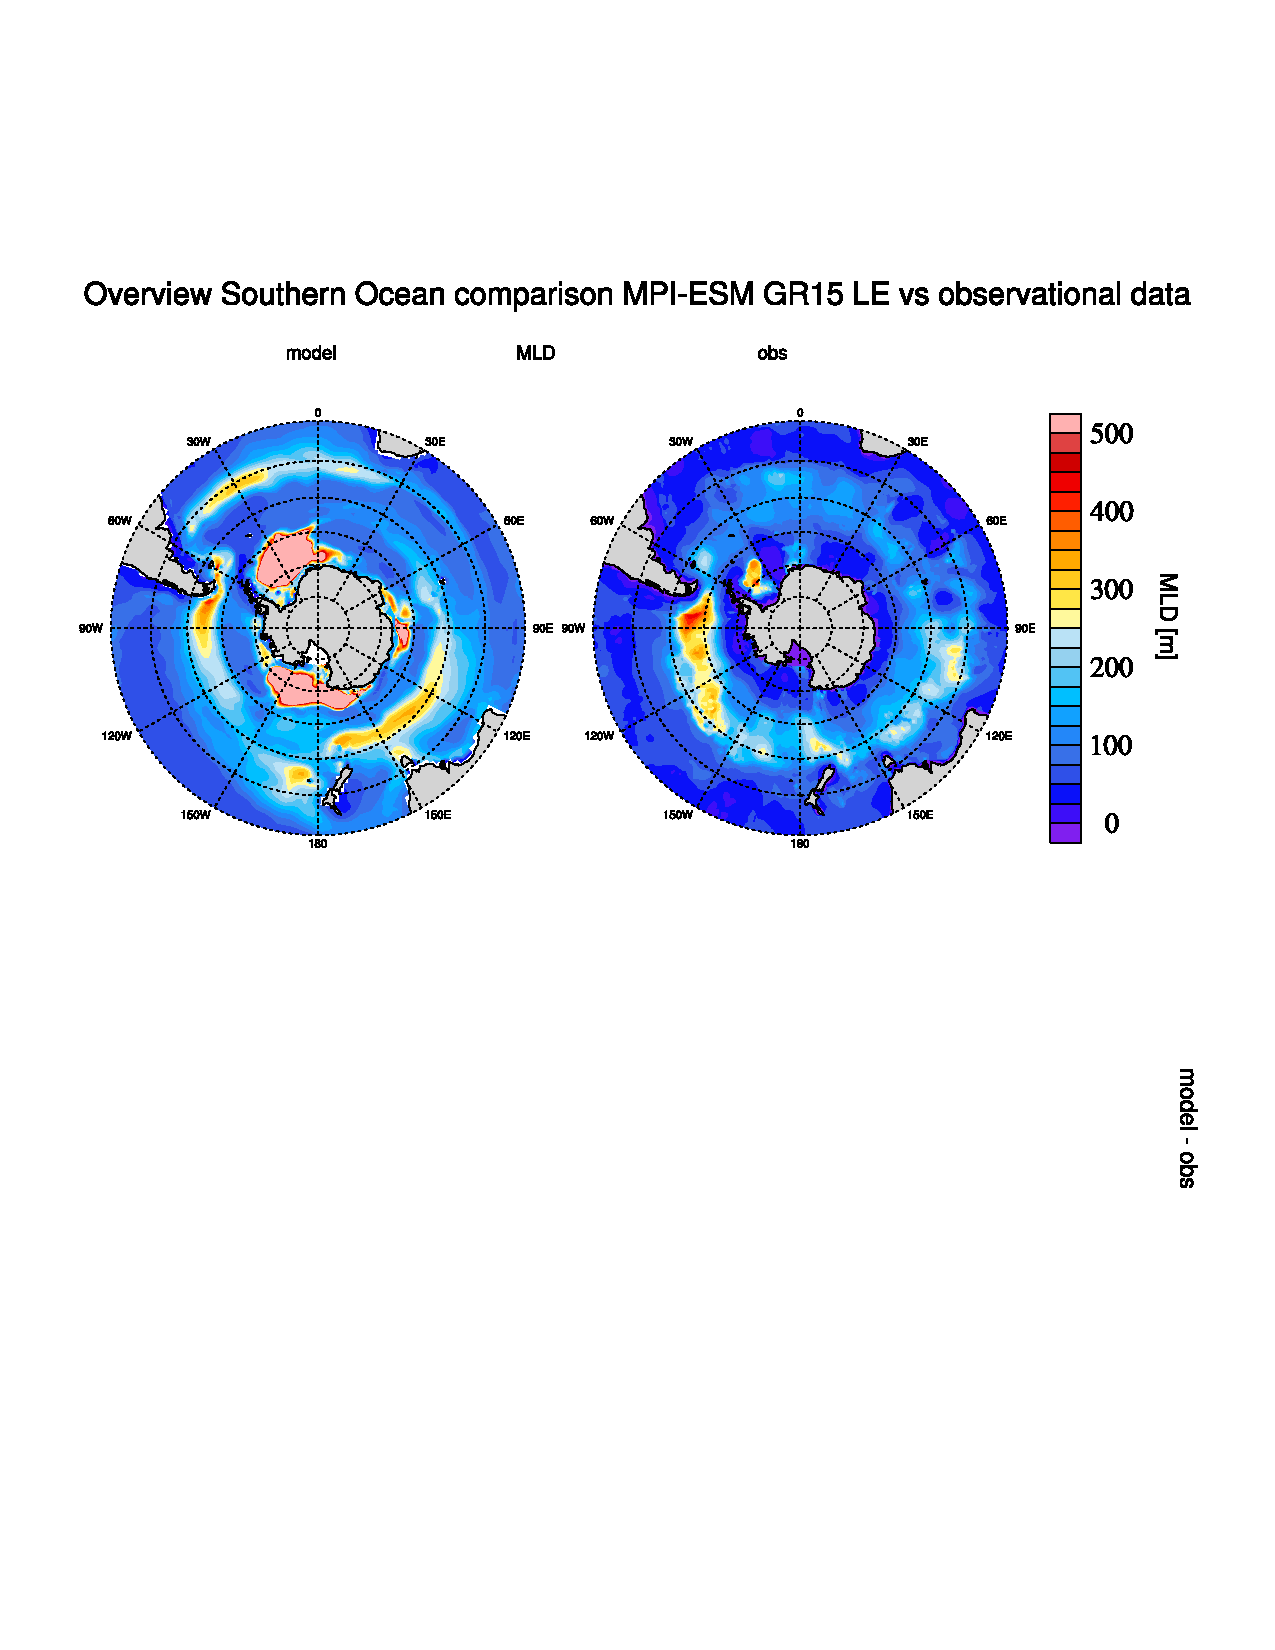
\includegraphics[scale=.85,page=1,trim=1.8cm 13.3cm .8cm 6.5cm,clip]{Overview_SO_MPIOM_comparison.pdf} % zmld
	\caption{Spatial distribution of the ensemble mean climatology (1980-2004) of the mixed-layer depth (MLD) (left) compared with Monterey \& Levitus, 1997 NOAA Atlas}
	\label{fig:SO_comp_zmld}
\end{figure}


%\paragraph{what I could add: globalMOC. The carbon trends have opposing MOC trends. Should I?}





\clearpage

\section{Trends in CO$_2$ flux}
\label{ch:trends}

\subsection{Winds determine internal variability of the Southern Ocean CO$_2$ flux}

%\paragraph{on area 50-60S as driver of Southern Ocean internal variability, correlation plots co2flux and wind trends} 
I find a correlation on 8-year trends between SAM, which describes the position and latitudinal shift of westerly winds, and the CO$_2$ flux in the area of largest decadal internal variability at 50-60$^\circ$S (fig. \ref{fig:scatter}). Although the CO$_2$ flux formula depends on the wind speed at 10m height, figure \ref{fig:scatter} emphasizes the importance and the changes in $\Delta \text{pCO}_2$. However, the magnitude of short-term variability on the timescale of days to hours depends highly on wind strength variability, but the direction of CO$_2$ flux is independent of wind speed. This relationship reveals two distinct regimes of wind-driven CO$_2$ flux signals in this area: 

Intensified and southward shifted winds, associated with an increasing trend in SAM, lead to a positive CO$_2$ flux trend. This Southern Ocean carbon sink response has been suggested frequently for the observed and projected trend in SAM \citep{LeQuere2007,Lovenduski2007,Lovenduski2008,Hauck2013}. The related processes associated stronger winds are explained in section \ref{sec:trends_pos}.

In MPI-ESM we also find the reverse case of weakening and northward shifting winds, associated with a negative trend in SAM, which lead to a negative CO$_2$ flux or ocean uptake trend. The related processes associated weaker winds are explained in section \ref{sec:trends_neg}. However, observations do not reveal strong multi-year negative SAM trends (see fig. \ref{fig:evolution_SAM}). Likewise, westerly winds did not weaken but continued to increase during the negative CO$_2$ flux trend in the 2000s \citep{landschuetzer2015}. \newline


\begin{figure}[h!]
\centering
%		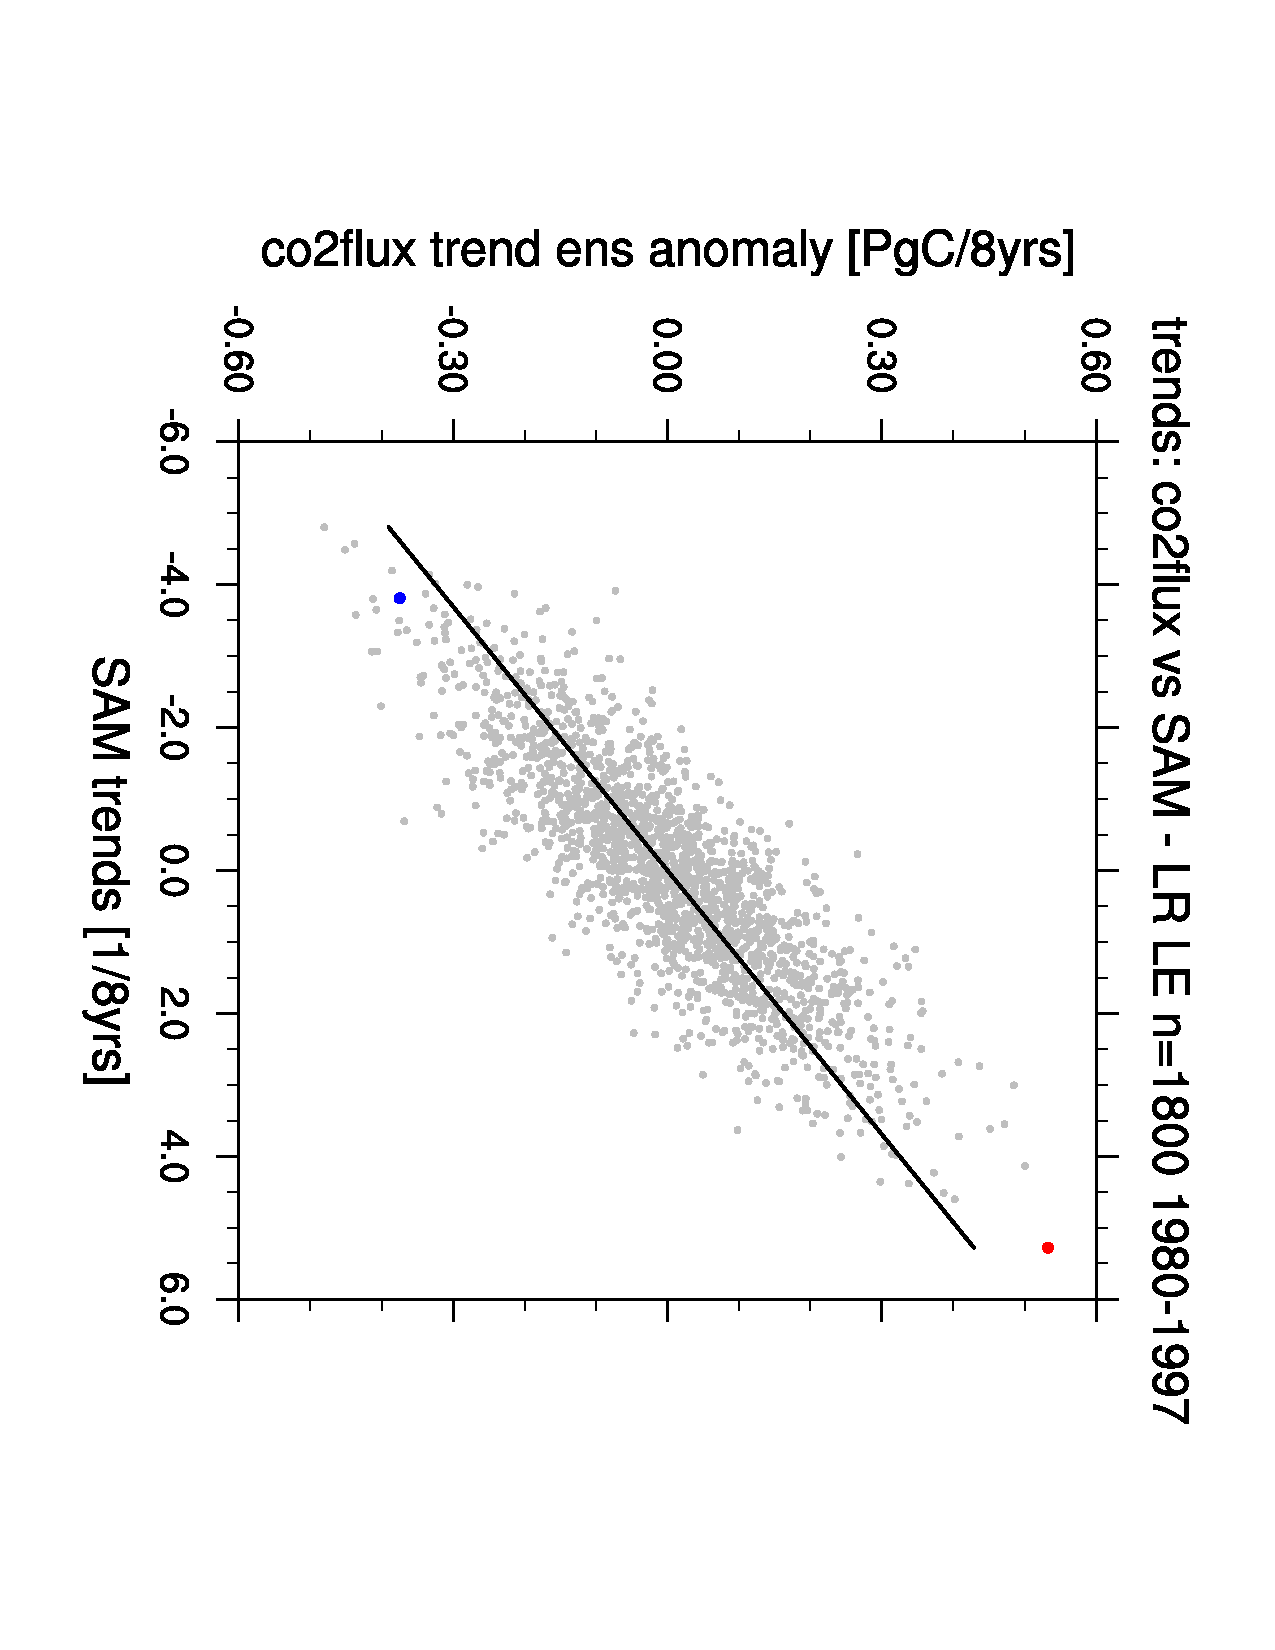
\includegraphics[scale=.5,page=1,angle=90,trim=1.3cm 2.3cm 2.3cm 3cm,clip]{Scatter_trends_bands_ensanom_co2flux_vs_SAM_n1800_1980_1997_trend8_50-59S}
		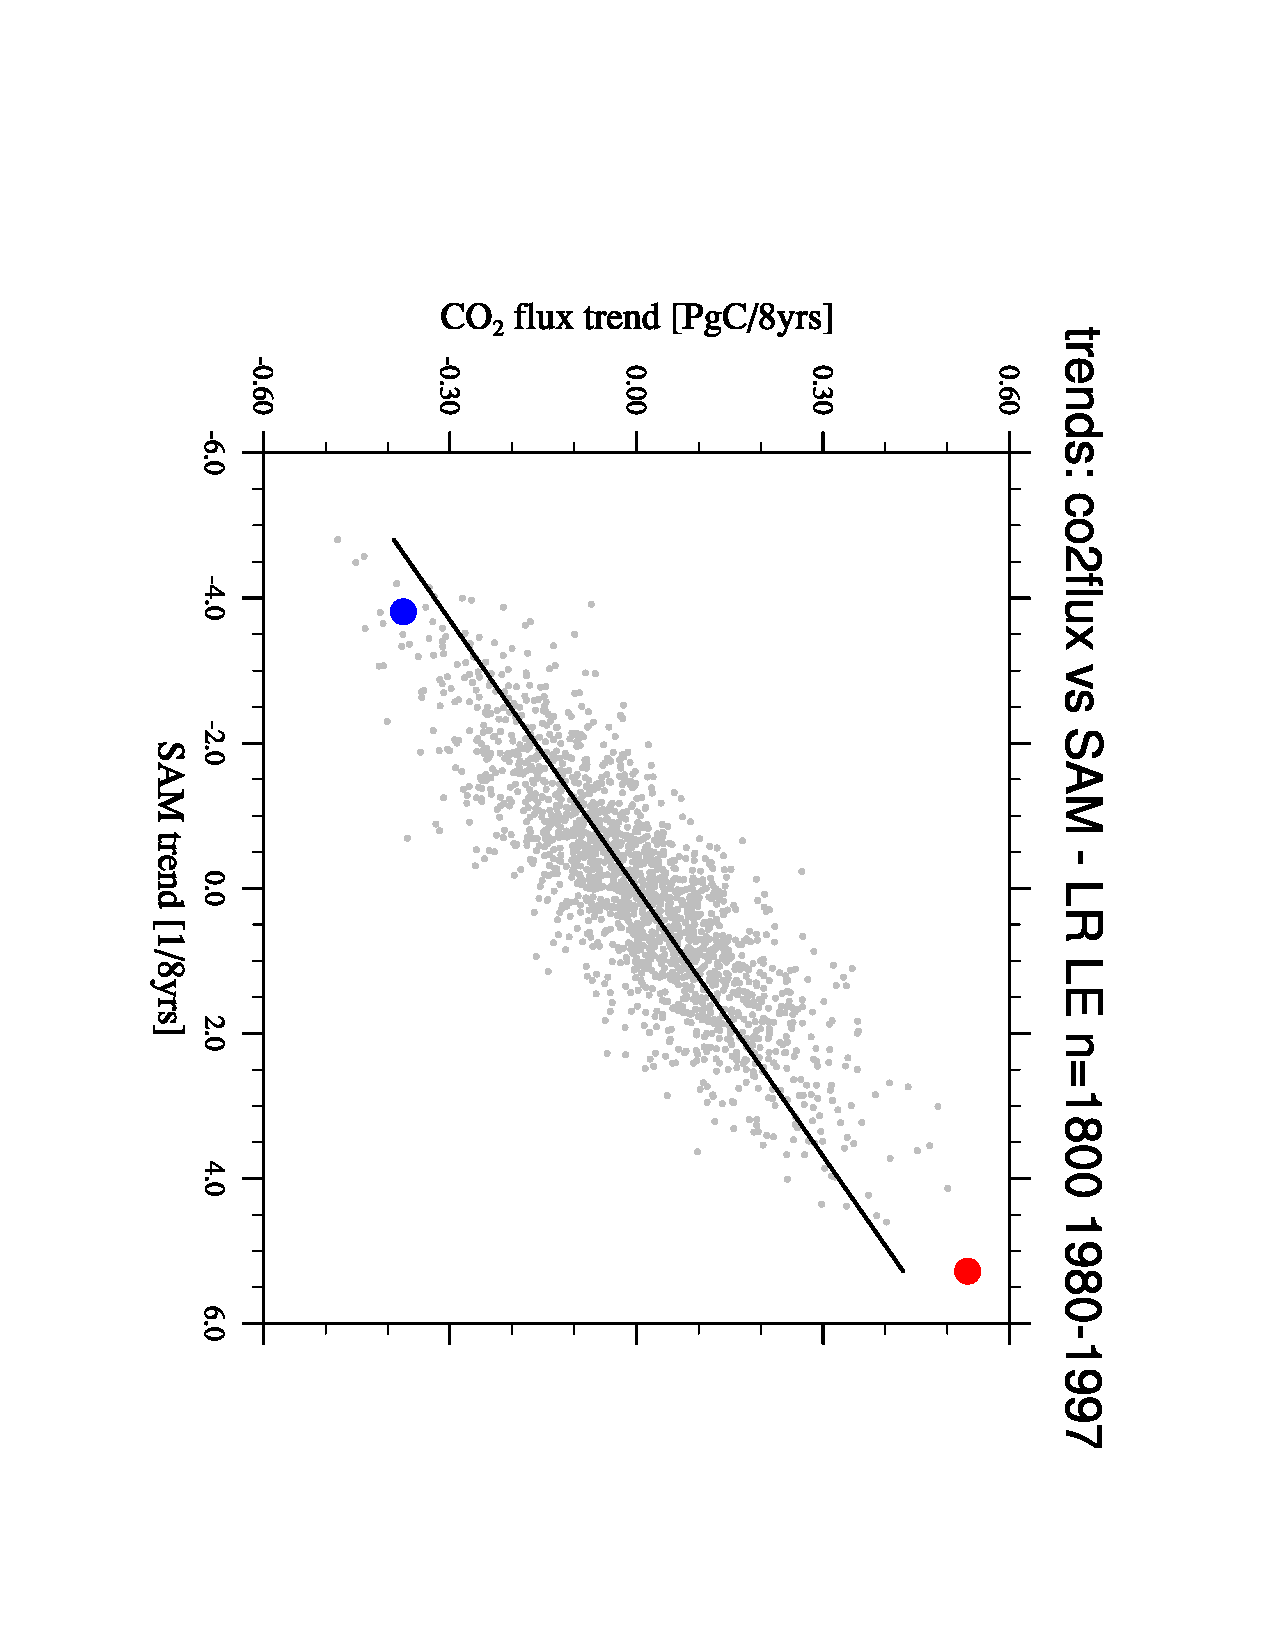
\includegraphics[scale=.5,page=1,angle=90,trim=1.3cm 2.3cm 3.8cm 3cm,clip]{EGU_new_SAM_Scatter_trends_bands_ensanom_co2flux_vs_SAM_n1800_1980_1997_trend8}
		
		%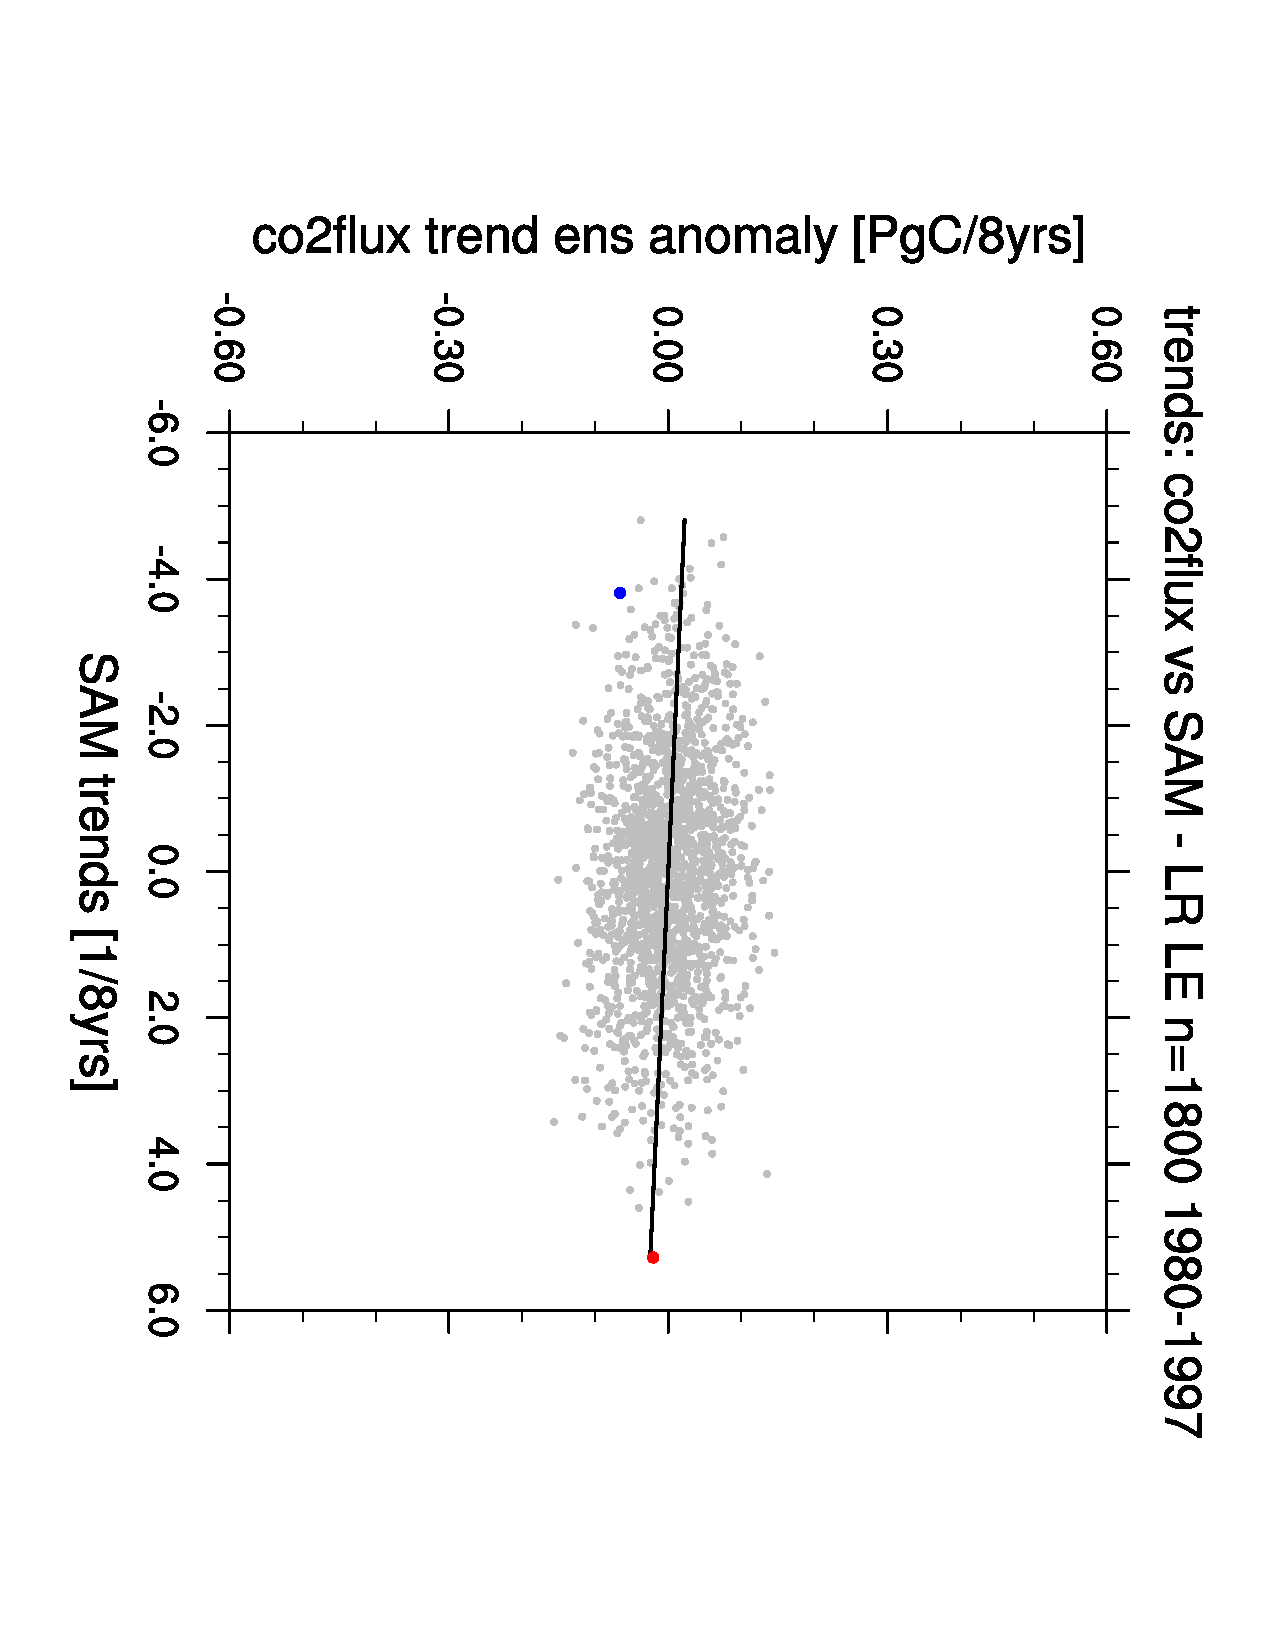
\includegraphics[scale=.38,page=1,angle=90,trim=1.3cm 2.3cm 2.3cm 3cm,clip]{Scatter_trends_bands_ensanom_co2flux_vs_SAM_n1800_1980_1997_trend8_40-49S}
		\vspace{-2mm}
		\caption{Linear trends in the Southern Annular Mode (SAM) as indicator of wind strength vs. CO$_2$ flux at 50-60$^\circ$S; each data point represents 8-year trends of a single realization normalized for the ensemble mean trend  between 1980 and 2005; the blue dot is the most negative monotonic CO$_2$ flux trend; the red dot is positive monotonic CO$_2$ flux trend.}
		\label{fig:scatter}
\end{figure}

To qualitatively understand the mechanisms of the Southern Ocean carbon sink, I analyze the drivers of CO$_2$ flux on a process level. This chapter covers CO$_2$ flux changes with respect to the thermal effect, physical circulation and biology. A quantitative analysis of the different drivers for different regions discussed in chapter \ref{ch:pCO2separation}.

The analysis presented here involves 8-year trends for reasons stated in section \ref{sec:choicetrend}, but the results of this chapter apply to various multi-year trends subject to internal variability (not shown).

The spatial trend patterns of different trend periods appear zonally symmetric, therefore the analysis is not separated into the different Southern Ocean sectors, e.g. Pacific, Indian or Atlantic. Also, the atmospheric circulation change in models are too symmetric compared to observations \citep{Haumann2014}. Therefore, the description here is carried out in zonal latitudinal bands keeping the unsymmetrical Southern Ocean dynamics in mind \citep{Sallee2010,Talley2013}. Also due to the underestimated Antarctic sea-ice and open-ocean convection in the Ross and Weddell Sea, I restrict my analysis to the Southern Ocean north of 60$^\circ$S, but the decadal CO$_2$ flux trends have a weak signal south of 60$^\circ$S anyway. 



\clearpage

\subsection{Positive CO$_2$ flux trends}
\label{sec:trends_pos}

Strong positive CO$_2$ flux trends correlate with stronger westerly winds (fig. \ref{fig:scatter}). The difference $\Delta$pCO$_2$ between oceanic pCO$_{2,\text{ocean}}$ and atmospheric partial pressures pCO$_{2,\text{atm}}$ depicts a cleaner signal than CO$_2$ flux and is independent of wind speed. pCO$_{2,\text{ocean}}$ rises stronger than pCO$_{2,\text{atm}}$, so CO$_2$ must be driven by changes in the ocean dynamics (fig. \ref{fig:pco2_pos}a).
The strongest positive signal occurs in the upwelling at 50-60$^\circ$S, a weaker and more patchy signal occurs in the subduction areas north of 50$^\circ$S, whereas changes in most other areas of the Southern Ocean are insignificant (fig. \ref{fig:pco2_pos}a). 

Westerly winds decrease at 40-50$^\circ$S and increase at 50-60$^\circ$S which results in a southward shift of westerlies (fig. \ref{fig:pco2_pos}b) represented by the positive trend in SAM (see fig. \ref{fig:evolution_SAM}). \newline


The response of the thermal effect, upper-ocean overturning circulation and biology are described in sections \ref{sec:trends_pos_thermal}, \ref{sec:trends_pos_circulation} and \ref{sec:trends_pos_biology}, respectively.


\begin{figure}[h!]
\centering
	\includegraphics[scale=.8,trim=6.3cm 14.4cm 5.5cm 6.4cm,clip]{\memberpositive _positive_trend_8_Landschuetzer_overview.pdf}
	\includegraphics[scale=1.05,trim=7.2cm 4.7cm 6.8cm 17.8cm,clip]{\memberpositive _positive_trend_8_Landschuetzer_overview.pdf}	
	\caption{Linear trends in $\Delta$pCO$_2$ (left) and sea-level pressure and wind vectors overlain as arrows (right) for the case of the most positive monotonic 8-year CO$_2$ flux trend; hatched areas indicate where trends are outside the 5\% significance level}% - should I also discuss thermal and non-thermal trends in \citep{landschuetzer2015}?}
	\label{fig:pco2_pos}
\end{figure}






\clearpage

\subsubsection{Changes in the thermal effect in positive CO$_2$ flux trends}
\label{sec:trends_pos_thermal}

The difference between the partial pressure of CO$_2$ in oceanic pCO$_{2,\text{ocean}}$ and atmospheric pCO$_{2,\text{atm}}$ is the main changing quantity in the CO$_2$ flux formula. The separation by \cite{Takahashi2002} gives insights about the direct influence of sea-surface temperatures (SST) (see section \ref{sec:takahashi}). The thermal pCO$_2$ trend is driven by changes in SST (fig. \ref{fig:thermal_pos}a), whereas the non-thermal trend includes changes in pCO$_{2,\text{atm}}$, biology, alkalinity, at constant SST (fig. \ref{fig:thermal_pos}b). The thermal trend and non-thermal trend approximately add up to the trends in pCO$_2$ \citep{landschuetzer2015}.

The thermal trend follows the SST cooling trend (fig. \ref{fig:sst_pos}) south of 50$^\circ$S towards negative CO$_2$ flux trends, whereas the warming north of 50$^\circ$S favors outgassing. Increased Ekman transport causes this heat divergence in polar regions and a heat convergence at lower latitudes, which cause this response in the thermal pump \citep{Hall2002} (see fig. \ref{fig:UOOC_pos}). The non-thermal component strongly increases south of 50$^\circ$S, so overall the pCO$_{2,\text{ocean}}$ increases faster than pCO$_{2,\text{atm}}$, which leads to a positive CO$_2$. This reflects the enhanced outgassing from increased upwelling. The non-thermal and thermal trends combined nearly compensate north of 50$^\circ$S, but at 50-60$^\circ$S the outgassing dominates (fig. \ref{fig:pco2_pos}a). The homogenous increase in atmospheric pCO$_{\text{2,atm}}$ accounts for a -12ppm/8yrs in fig. \ref{fig:pco2_pos}b. 
These changes are stronger in the summer season, especially the non-thermal component (see fig. \ref{fig:thermal_pos_summer}, \ref{fig:thermal_pos_winter}). 

\begin{figure}[h!]
\centering
	\includegraphics[scale=1.6,trim=6cm 10.2cm 5.2cm 14cm,clip]{\memberpositive _positive_trend_8_Landschuetzer_overview.pdf}
	\caption{Linear trends in pCO$_{2,\text{thermal}}$ (left) and $\Delta$pCO$_{2,\text{non-thermal}}$ (right) for the case of the most positive monotonic 8-year CO$_2$ flux trend; hatched areas indicate where trends are outside the 5\% significance level}
	\label{fig:thermal_pos}
\end{figure}



\clearpage

\subsubsection{Changes in ocean circulation in positive CO$_2$ flux trends}
\label{sec:trends_pos_circulation}

Stronger westerly winds intensify the upper-ocean overturning circulation \citep{Lauderdale2013}. The circulation field advects DIC along its overturning pathway (fig. \ref{fig:UOOC_pos}). Intensified upwelling of carbon-rich waters 50-60$^\circ$S increases DIC concentrations in the euphotic zone (fig. \ref{fig:ekman_pos}b). An over-saturation in DIC leads to a positive CO$_2$ flux. The stronger winds also increase Ekman northward transport and advects DIC further northward (fig. \ref{fig:ekman_pos}a). North of 50$^\circ$S, subduction rates of AAIW and SAMW formation increase, so pCO$_{2,\text{atm}}$-equilibrated waters take additional anthropogenic carbon into the deeper ocean. The southward shift of westerly winds weakens the northern edge of Ekman transport at 30-40$^\circ$S. 

The changes in mixed-layer depth (MLD) also contribute to the vertical transport of carbon. By deeper mixing in winter, more carbon-rich waters are included in the MLD, which then serves as a larger reservoir of super-saturated DIC. MLD deepens south of 50$^\circ$S and slightly shoals north of 45$^\circ$S, whereas open-ocean convection causes the unrealistic zonal MLD averages below 300m south of 60$^\circ$S (fig. \ref{fig:UOOC_pos}) (\citep{Sallee2013,Stoessel2015}). 


\begin{figure}[h!]
	\centering
	\includegraphics[scale=1.45,trim=13.cm 18.75cm 3cm 6cm,clip]{\memberpositive _positive_trend_8_ekman_overview.pdf}
	\includegraphics[scale=1.45,trim=13.25cm 15.9cm 3cm 9.2cm,clip]{\memberpositive _positive_trend_8_ekman_overview.pdf}
	\vspace{-5mm}
	\caption{Linear trends in Ekman transport and Ekman pumping in the case of the most positive 8-years CO$_2$ flux trend; hatched areas indicate where trends are outside the 5\% significance level}
	\label{fig:ekman_pos}
\end{figure}


\begin{figure}[h!]
	\centering
	\includegraphics[scale=0.55,page=2,trim=.3cm 1.7cm 0cm 4.6cm,clip]{UOOC}
	\vspace{-5mm}
	\caption{Zonally averaged upper-ocean overturning circulation in the case of the most positive 8-year CO$_2$ flux trend; black arrows show mean advective carbon transport, red arrows show positive advective carbon transport trends; blue arrows show negative advective carbon transport trends; black numbers quantify the trends in advective carbon transport in PgC/8yrs; white lines are isopyncals as in fig. \ref{fig:UOOC_mean}; grey line is mixed-layer depth (MLD) in the beginning and the black line MLD in the end of the period.}
	\label{fig:UOOC_pos}
\end{figure}

The upper-ocean overturning circulation response presented here is in line with idealized wind-change studies \citep{Lauderdale2013}, modeling studies explaining the observed CO$_2$ flux trend in the 1990s \citep{LeQuere2007,Lovenduski2007,Lovenduski2008}, as well an inverse modeling study for the 1990s \citep{DeVries2017}.



\clearpage

\subsubsection{Changes in biology in positive CO$_2$ flux trends}
\label{sec:trends_pos_biology}
The biological pump draws down surface DIC and is sensitive to changes in circulation (see section \ref{sec:HAMOCC}). In this subsection, I analyze the 8-year summer (SONDJF) austral summer trends of quantities related to primary production. 
  
Primary production and CO$_2$ flux show opposing zonally symmetric trend patterns as phytoplankton growth takes up large amounts of surface DIC and hence lowers pCO$_2$ (fig. \ref{fig:summer_trends_pos}a,b). Primary production declines most pronounced at 50-60$^\circ$S, increases at 40-50$^\circ$S and declines at 30-40$^\circ$S. Why?
%\paragraph{on intpp not increasing because of more nutrients} different than \citep{Lovenduski2005} 

Internal variability might change the availability of nutrients. 
The decline in nutrients in the subtropics at 30-40$^\circ$S reduces primary production, but the nutrient availability factor (for definition see \ref{sec:HAMOCC}) slightly increases south of 50$^\circ$S (fig. \ref{fig:summer_trends_pos}c).
Previous observational and modeling studies suggest an increase in primary production, because upwelling brings nutrients, especially iron, from the deep-ocean to the iron-limited surface waters \citep{Lovenduski2005,Hauck2013,wang2012,Tagliabue2014}. Additional iron fosters primary production following the iron-hypothesis \citep{Martin1990Nature,Martin1990}, but observational data for iron is very sparse to test this for the whole Southern Ocean \citep{Tagliabue2014}. Contrasting HAMOCC, many models reproduce this suggested iron-limitation in the Southern Ocean and hence respond with increase primary production \citep{wang2012,Hauck2013}.  \newline

If the reduction in primary production at 50-60$^\circ$S cannot be explained by changes in nutrients, what else effects primary production blooms?

The combined light \& temperature limitation is primarily driven by temperature after the insulation excels a threshold in cold waters (see fig. \ref{fig:lighttemplimf}). A strong SST cooling trend comes along with stronger winds, because the increased Ekman transport pushes cold polar waters more northward (fig. \ref{fig:sst_pos}). The strong light \& temperature limitation signal in coastal areas as well as Weddell and Ross Sea is attributed to sea-ice changes and open-ocean convection, but has minor effects on the primary production and CO$_2$ flux (fig. \ref{fig:summer_trends_pos}d). 

This northward Ekman transport could also advect phytoplankton northwards to cause the increase in primary production at 40-50$^\circ$S (fig. \ref{fig:ekman_pos}).

The overall decline of primary production in the Southern Ocean under a positive SAM trend is related to mixing:
The summer mixed-layer depth (MLD) has a strong increasing trend at 50-60$^\circ$S, so the mixing deepens (fig. \ref{fig:summer_trends_pos}e). This is caused by stronger winds (fig. \ref{fig:pco2_pos}b) and shown in the average depth of the vertical diffusivity due to wind (fig. \ref{fig:summer_trends_pos}f). This deeper mixing in summer then mixes the standing stock of phytoplankton to deeper levels, where they are exposed to less light (fig. \ref{fig:summer_trends_pos}g). This theory of a critical depth for phytoplankton blooms was proposed by \cite{Sverdrup1953} and requires a stable water column for phytoplankton to initiate blooms. However, this theory is based on turbulent mixing, so the oceanographic MLD only serves as a first-order mixing measure for phytoplankton \citep{Franks2014}. Still the signal sustains to phytoplankton depth, where the average phytoplankton depth decreases up to 15m which results in up to 30\% less light. The lack of monthly output for 3D biogeochemical variables made me use annual averages for phytoplankton, which causes the low significance in fig. \ref{fig:summer_trends_pos}g. 

The reverse processes contributes to the increase at 40-50$^\circ$S: Less winds mix less deep and allow phytoplankton to stay more confined to the surface, where they get more light and flurish (fig. \ref{fig:pco2_pos}b, \ref{fig:summer_trends_pos}e,f,g,b). Also the warming increases the phytoplankton growth rate (fig. \ref{fig:summer_trends_pos}d).
\\

Summarizing, a multitude of interconnected processes causes the decline in primary production in the Southern Ocean for an increasing SAM trend. A clear separation of the magnitude of the different effects is impossible.
 
%\llap{ \parbox[b]{8.0cm}{\textbf{a}\\\rule{0ex}{3.7cm}}} %http://tex.stackexchange.com/questions/128844/put-subfigure-labels-inside-figures-using-subfig-package
%%%	\llap{ \parbox[b]{.5cm}{\textbf{b}\\\rule{0ex}{3.7cm}}}	

\begin{figure}[h!] %lbrt
	\includegraphics[scale=1.6,trim=13.2cm 18.75cm 3.4cm 6.3cm,clip]{\memberpositive _positive_trend_8_obgc_overview_summer.pdf} %co2flux
	\includegraphics[scale=1.6,trim=13.2cm 15.9cm 3.4cm 9.225cm,clip]{\memberpositive _positive_trend_8_obgc_overview_summer.pdf} %intpp
	\includegraphics[scale=1.6,trim=13.2cm 13.05cm 3.4cm 12.075cm,clip]{\memberpositive _positive_trend_8_obgc_overview_summer.pdf} %nutlimf
	\includegraphics[scale=1.6,trim=13.2cm 4.5cm 3.4cm 20.65cm,clip]{\memberpositive _positive_trend_8_obgc_overview_summer.pdf} %light_temp	
	\includegraphics[scale=1.6,trim=13.2cm 7.3cm 3.4cm 17.775cm,clip]{\memberpositive _positive_trend_8_obgc_overview_summer.pdf} %zmld
	\includegraphics[scale=1.6,trim=13.2cm 15.9cm 3.4cm 9.2cm,clip]{\memberpositive _positive_trend_8_schwerpunkt_mixing_overview.pdf} % wind penetration depth	
	\includegraphics[scale=1.6,trim=13.2cm 18.7cm 3.4cm 6.4cm,clip]{\memberpositive _positive_trend_8_schwerpunkt_mixing_overview.pdf} % phy depth	

	\caption{Southern Ocean austral summer trends for the case of the most positive 8-year CO$_2$ flux trend: CO$_2$ flux (a), vertically integrated primary production (b), nutrient availability factor (c), surface temperature \& limitation function (d), mixed layer depth (e); average depth of vertical diffusivity due to wind (f) and phytoplankton average depth (g); hatched areas indicate where trends are outside the 5\% significance level}
	\label{fig:summer_trends_pos}
\end{figure}



\clearpage



\subsection{Negative CO$_2$ flux trends}
\label{sec:trends_neg}

Disclaimer: Generally, trends in this analysis reverse for weaker compared to strengthening westerlies, which leads to an overall negative CO$_2$ flux trend. Additionally, now the prescribed atmospheric $pCO_{2,\text{atm}}$ forcing promotes a steady negative background CO$_2$ flux trend.\newline

Strong negative CO$_2$ flux trends correlate with weaker westerly winds (fig. \ref{fig:pco2_neg}). The strongest negative signal $\Delta$pCO$_2$ occurs in the upwelling at 50-60$^\circ$S, whereas changes in most other areas of the Southern Ocean are insignificant (fig. \ref{fig:pco2_neg}a). 

Westerly winds decrease at 40-60$^\circ$S, which results in a northward shift of westerlies (fig. \ref{fig:pco2_pos}) represented by the negative trend in SAM (see fig. \ref{fig:evolution_SAM}).
\\

%The strengthening of the Southern Ocean carbon sink under the context of intensified westerly winds leads me to a hypothesis (fig. \ref{fig:schematics_pos}):
%Weaker winds at 50-60$^\circ$S slow down the upper-ocean overturning circulation and increase primary production due to a more stable water column. [really unsure about this hypothesis part - I dont discover anything new but want to explain the process with a figure ahead]
The response in the thermal effect, upper-ocean overturning circulation and biology are described in sections \ref{sec:trends_neg_thermal}, \ref{sec:trends_neg_circulation} and \ref{sec:trends_neg_biology}, respectively.


\begin{figure}[h!]
\centering
	\includegraphics[scale=.8,trim=6.3cm 14.4cm 5.5cm 6.4cm,clip]{\membernegative _positive_trend_8_Landschuetzer_overview.pdf}
	\includegraphics[scale=1.05,trim=7.2cm 4.7cm 6.8cm 17.8cm,clip]{\membernegative _positive_trend_8_Landschuetzer_overview.pdf}	
	\caption{Linear trends in $\Delta$pCO$_2$ (left) and sea-level pressure and wind vectors overlain as arrows (right) for the case of the most negative monotonic 8-year CO$_2$ flux trend; hatched areas indicate where trends are outside the 5\% significance level}
	\label{fig:pco2_neg}
\end{figure}

\clearpage

\subsubsection{Changes in the thermal effect in negative CO$_2$ flux trends}
\label{sec:trends_neg_thermal}

The thermal trend follows the SST warming trend (fig. \ref{fig:sst_neg}) south of 50$^\circ$S towards positive CO$_2$ flux trends, whereas the cooling north of 50$^\circ$S favors CO$_2$ uptake (fig. \ref{fig:thermal_neg}a). This is caused by a heat convergence in the polar region and a heat divergence in the subtropics caused by less Ekman transport \citep{Hall2002}. The non-thermal trend is slightly positive north of 50$^\circ$S and negative south of 50$^\circ$S with the strongest signal in the areas of upwelling at 50-60$^\circ$S (fig. \ref{fig:thermal_neg}b). The increase in atmospheric pCO$_{\text{2,atm}}$ accounts for a -14ppm/8yrs. The non-thermal and thermal trends combined nearly compensate  north of 50$^\circ$S, but the non-thermal component dominates at 50-60$^\circ$S (fig. \ref{fig:pco2_neg}a). 

These changes are stronger in the summer season, especially the non-thermal component (see fig. \ref{fig:thermal_neg_summer}, \ref{fig:thermal_neg_winter}). 

\begin{figure}[h!]
\centering
	\includegraphics[scale=1.6,trim=6cm 10.2cm 5.2cm 14cm,clip]{\membernegative _positive_trend_8_Landschuetzer_overview.pdf}
	\caption{Linear trends in pCO$_{2,\text{thermal}}$ (left) and $\Delta$pCO$_{2,\text{non-thermal}}$ (right) for the case of the most negative monotonic 8-year CO$_2$ flux trend; hatched areas indicate where trends are outside the 5\% significance level}
	\label{fig:thermal_neg}
\end{figure}
 





\clearpage

\subsubsection{Changes in ocean circulation in negative CO$_2$ flux trends}
\label{sec:trends_neg_circulation}

Weaker westerly winds slow down the upper-ocean overturning circulation \citep{Lauderdale2013}. The circulation field advects DIC along its overturning pathway (fig. \ref{fig:UOOC_neg}). Weaker upwelling of carbon-rich waters 50-60$^\circ$S decreases DIC concentrations in the euphotic zone (fig. \ref{fig:ekman_neg}b). An under-saturation in DIC leads to a negative CO$_2$ flux. Weaker winds also decrease Ekman northward transport and advects DIC less northward (fig. \ref{fig:ekman_neg}a). North of 50$^\circ$S, subduction rates of AAIW and SAMW formation decrease, so pCO$_{2,\text{atm}}$-equilibrated waters take less anthropogenic carbon into the deeper ocean. The northward shift of westerly winds strengthens the northern edge of Ekman transport at 30$^\circ$S. MLD shoals south of 50$^\circ$S and slightly deepens north of 45$^\circ$S, whereas open-ocean convection causes the unrealistic zonal MLD averages below 300m south of 60$^\circ$S  (fig. \ref{fig:UOOC_neg}). 


\begin{figure}[h!]
	\centering
	\includegraphics[scale=1.45,trim=13.cm 18.75cm 3cm 6cm,clip]{\membernegative _positive_trend_8_ekman_overview.pdf}
	\includegraphics[scale=1.45,trim=13.25cm 15.9cm 3cm 9.2cm,clip]{\membernegative _positive_trend_8_ekman_overview.pdf}
	\vspace{-5mm}
	\caption{Linear trends in Ekman transport and Ekman pumping in the case of the most negative 8-years CO$_2$ flux trend; hatched areas indicate where trends are outside the 5\% significance level}
	\label{fig:ekman_neg}
\end{figure}


\begin{figure}[h!]
	\centering
	\includegraphics[scale=0.55,page=3,trim=.3cm 1.7cm 0cm 4.cm,clip]{UOOC}
	%\includegraphics[scale=0.5,page=3,trim=1.4cm 1.7cm 0cm 4.6cm,clip]{UOOC}
	\vspace{-10mm}
	\caption{Zonally averaged upper-ocean overturning circulation in the case of the most negative 8-year CO$_2$ flux trend; black arrows show mean advective carbon transport, red arrows show positive advective carbon transport trends; blue arrows show negative advective carbon transport trends; black numbers show the trends in advective carbon transport in PgC/8yrs; white lines are isopyncals as in fig. \ref{fig:UOOC_mean}; grey line is mixed-layer depth (MLD) in the beginning and the black line MLD in the end of the period.}%; black arrows show mean advective carbon transport, red arrows show advective carbon transport trend over 8 years; white lines are isopyncals separating Sub-Antarctic Mode Water (SAMW), Antarctic Intermediate Water (AAIW), Circumpolar Deep Water (CDW) and Antarctic Bottom Water (AABW)}
	\label{fig:UOOC_neg}
\end{figure}


The upper-ocean overturning circulation response presented here is in line with idealized wind-change studies \citep{Lauderdale2013}. The inverse modeling study reports a decline from the 2000s towards the previous decade \citep{DeVries2017}. However, a negative trend for the strength of westerly winds has not been observed, but the patterns in sea-level pressure in the 2000s became more zonally asymmetric \citep{landschuetzer2015}.


\clearpage

\subsubsection{Changes in biology in negative CO$_2$ flux trends}
\label{sec:trends_neg_biology}


%The biological pump draws down surface DIC and sensitive to changes in circulation (see section \ref{sec:HAMOCC}). In this subsection, I analyze the 8-year summer (SONDJF) austral summer trends. 
  
Primary production and CO$_2$ flux show opposing zonally symmetric trend patterns as phytoplankton growth takes up large amounts of surface DIC and hence lowers pCO$_2$ (fig. \ref{fig:summer_trends_neg}a,b). CO$_2$ flux trend here also follows the atmospheric pCO$_{2,\text{atm}}$ forcing. Primary production increases most pronounced at 50-60$^\circ$S, decreases at 40-50$^\circ$S and increases at 30-40$^\circ$S. Why?
%\paragraph{on intpp not increasing because of more nutrients} different than \citep{Lovenduski2005} 

Internal variability might change the availability of nutrients. 
The increase in nutrients in the subtropics at 30-40$^\circ$S fosters primary production, but nutrient availability factor slightly decreases south of 50$^\circ$S (fig. \ref{fig:summer_trends_neg}c). 
Previous observational and modeling studies suggest an decrease in primary production because less upwelling brings less nutrients, especially iron, from the deep-ocean to the surface \citep{Tagliabue2014}. But the Southern Ocean in HAMOCC is nitrate limited, so the slight nutrient depletion might originate in the increases nutrient consumption due to primary production.  \newline

If the reduction in primary production at 50-60$^\circ$S cannot be explained by changes in nutrients, what else effects primary production blooms?

A strong SST warming trend comes along with weaker winds, because the increased Ekman transport pushes cold polar waters less northward (fig. \ref{fig:sst_neg}). The strong light \& temperature limitation signal in coastal areas as well as Weddell and Ross Sea is attributed to sea-ice changes and open-ocean convection, but has minor effects on the primary production and CO$_2$ flux (fig. \ref{fig:summer_trends_neg}d). 

The weakened northward Ekman transport could also keep the phytoplankton more southwards and cause the increase in primary production at 50-60$^\circ$S and the shifted decrease at 40-50$^\circ$S (fig. \ref{fig:ekman_neg}).

The overall increase of primary production in the Southern Ocean under a positive SAM trend is also related to mixing:
The summer mixed-layer depth (MLD) has a strong decreasing trend at 50-60$^\circ$S, so the mixing decreases (fig. \ref{fig:summer_trends_neg}e). Weaker winds (fig. \ref{fig:pco2_neg}b) mix the ocean less deep (fig. \ref{fig:summer_trends_neg}f). This reduced mixing in summer keeps the standing stock of phytoplankton in light-flooded levels, where they grow faster (fig. \ref{fig:summer_trends_pos}g). 
The reverse process contributes to the decrease at 40-50$^\circ$S: Stronger winds mix deeper and draw phytoplankton down, where they get less light and grow less (fig. \ref{fig:pco2_pos}b, \ref{fig:summer_trends_pos}e,f,g,b). Additionally, the cooling slows down phytoplankton growth (fig. \ref{fig:summer_trends_neg}d).
\\

Summarizing, a multitude of interconnected processes caused the increase in primary production in the Southern Ocean for a decreasing SAM trend. A clear separation of the magnitude of the different effects is impossible.
 

\begin{figure}[h!]
	\includegraphics[scale=1.6,trim=13.2cm 18.75cm 3.4cm 6.3cm,clip]{\membernegative _positive_trend_8_obgc_overview_summer.pdf} %co2flux
	\includegraphics[scale=1.6,trim=13.2cm 15.9cm 3.4cm 9.225cm,clip]{\membernegative _positive_trend_8_obgc_overview_summer.pdf} %intpp
	\includegraphics[scale=1.6,trim=13.2cm 13.05cm 3.4cm 12.075cm,clip]{\membernegative _positive_trend_8_obgc_overview_summer.pdf} %nutlimf
	\includegraphics[scale=1.6,trim=13.2cm 4.5cm 3.4cm 20.65cm,clip]{\membernegative _positive_trend_8_obgc_overview_summer.pdf} %light_temp	
	\includegraphics[scale=1.6,trim=13.2cm 7.3cm 3.4cm 17.775cm,clip]{\membernegative _positive_trend_8_obgc_overview_summer.pdf} %zmld
	\includegraphics[scale=1.6,trim=13.2cm 15.9cm 3.4cm 9.2cm,clip]{\membernegative _positive_trend_8_schwerpunkt_mixing_overview.pdf} % wind penetration depth	
	\includegraphics[scale=1.6,trim=13.2cm 18.7cm 3.4cm 6.4cm,clip]{\membernegative _positive_trend_8_schwerpunkt_mixing_overview.pdf} % phy depth	

		\caption{Southern Ocean austral summer trends for the most negative 8-year CO$_2$ flux trend: CO$_2$ flux (a), vertically integrated primary production (b), nutrient availability factor (c), surface temperature \& limitation function (d), mixed layer depth (e); average depth of vertical diffusivity due to wind (f) and phytoplankton average depth (g); hatched areas indicate where trends are outside the 5\% significance level}
	\label{fig:summer_trends_neg}
\end{figure}



\clearpage
\section{Distinction of drivers in pCO$_2$}
\label{ch:pCO2separation}

\paragraph{Purpose of pCO$_2$ separation}
%\subsection{Explanation and assuof the framework and its assumptions}
The previous analysis of thermal, physical and biological controls of the Southern Ocean carbon sink asks for an estimate on the relative contributions of change. As the interconnected processes always influence and change each other directly, a clear and clean separation cannot be taken in precision, but rather for an \textit{estimate of the first-order drivers} in CO$_2$ flux. In this chapter, I adapt the pCO$_2$ diagnostics framework from \cite{Lovenduski2007} to quantitatively relate the different contributors to pCO$_{\text{2,ocean}}$ and hence CO$_2$ flux.

\subsection{Derivation of the framework}
The framework assumes an euphotic zone zonal carbon budget box where at the upper boundary CO$_2$ enters and at the lower boundary at the mixed-depth layer biology export production leaves the system (fig. \ref{fig:pCO2_separation}). Based on the individual processes taking place, a change in pCO$_2$ due to that process is calculated offline, i.e. from monthly model output data, instead of online, i.e. for each timestep when the model ran. \newline
\begin{figure}[h!]
	\centering
	\includegraphics[scale=.55,page=2,trim=5.cm 4.7cm 2.7cm 1.3cm,clip]{co2sep}
	\caption{Schematic illustration of pCO$_2$ driver separation assuming a well-mixed zonal carbon box of the upper-ocean, where CO$_2$ flux (red) is separated in contributions due to thermal (orange), freshwater (light blue), biology (green) and a residual for circulation (dark blue)}	
	\label{fig:pCO2_separation}
\end{figure}

I separate pCO$_2$ into contributions of temperature, salt, alkalinity and DIC. I use the salinity-normalized concentrations $(sDIC=\frac{DIC}{S}\cdot (S_0=35))$ for DIC and alkalinity to prevent double-accounting of freshwater changes in the DIC/alkalinity and salt contributions \citep{Keeling2004}.

\begin{align*}
\delta pCO_2&=\delta pCO_{\text{2,thermal}}+\delta pCO_{\text{2,salt}}+\delta pCO_{\text{2,alk}}+\delta pCO_{\text{2,DIC}} \\
&= \frac{\partial pCO_2}{\partial T}\delta T + \frac{\partial pCO_2}{\partial S}\delta S  + \frac{S}{S_0}\frac{\partial pCO_2}{\partial Alk}\delta sAlk  + \frac{S}{S_0}\frac{\partial pCO_2}{\partial DIC}\delta sDIC 
\end{align*}

\noindent The thermal separation is taken from \cite{Takahashi1993}:
\begin{align*}
\frac{\partial pCO_2}{\partial T} &\approx pCO_2 \cdot 0.0423 ^\circ C^{-1}  .
\end{align*}

\noindent The salinity, DIC and alkalinity contributions are taken from \cite{Sarmiento2006}:
\begin{align*}
\allowdisplaybreaks
\frac{\partial pCO_2}{\partial S} &\approx \frac{pCO_2}{S} \\
\frac{\partial pCO_2}{\partial DIC} &\approx \frac{pCO_2}{DIC} \cdot \gamma_{DIC} \\
\frac{\partial pCO_2}{\partial Alk} &\approx \frac{pCO_2}{Alk} \cdot \gamma_{Alk} \\
\gamma_{DIC} &\approx \frac{3 \cdot Alk \cdot DIC - 2 \cdot DIC^2}{(2 \cdot DIC - Alk)(Alk-DIC)} \\
\gamma_{Alk} &\approx -\frac{Alk^2}{(2 \cdot DIC - Alk)(Alk-DIC)}.
\end{align*}

\noindent Furthermore the changes in sDIC and sAlk are separated into biological, air-sea exchange or residual contribution:

\[\frac{\delta (sDIC)}{\delta t}=\frac{\delta (sDIC_{bio})}{\delta t}+\frac{\delta (sDIC_{exchange})}{\delta t}+\frac{\delta (sDIC_{residual})}{\delta t}.\]

\noindent The changes due to air-sea exchange and due to biology are converted to DIC and alkalinity changes by dividing by the mixed-layer depth (MLD) assumping a well-mixed mixed-layer depth. Furthermore, the effect of biological primary production contributes with organic patter production and calcium carbonate production to the sDIC changes and calcium carbonate alone accounts for changes in alkalinity.
\begin{align*}
sDIC_{bio}&=\frac{coex+caex}{MLD} \\
sDIC_{ex}&=\frac{CO_2flux}{MLD} \\
sAlk_{bio}&=\frac{caex}{MLD}
\end{align*}



This approach is based on the following assumptions:
\begin{itemize}
\item negligible error in approximations used during derivation
\item linearizations of non-linear processes
\item simplifications of buffering constants \citep{Sarmiento2006}
\item residual as combined contribution of [everything which is not described], mainly vertical and lateral circulation, but also to a lesser degree advection of biological constituents
\item no problem with monthly mean offline instead of instantaneous online values
\item well-mixed mixed layer
\end{itemize}

\clearpage
\subsection{Estimate of pCO$_2$ drivers}


Applying the above described framework yields an estimate for the drivers of pCO$_2$ for the two extreme trends (table \ref{tab:trends_pco2}).

In general, the trends reverse for opposite wind forcing and the area 50-60$^\circ$S sets the trend of the overall Southern Ocean carbon sink south of 35$^\circ$S. The changes in pCO$_2$ due to biology and temperature are much smaller than the residual circulation change. Biology seems more susceptible to wind-driven changes at 50-60$^\circ$S than 40-50$^\circ$S, this separation might be biased by the selection of the latitudinal boundaries.

In detail, the ongoing processes do not simply reverse as the atmospheric forcing trend stays the same. 
The most positive CO$_2$ flux trend is mainly driven by the non-thermal pCO$_{\text{2,ocean}}$ ocean changes, whereas the most negative CO$_2$ flux trend is mainly driven by the increasing pCO$_{\text{2,atm}}$ concentrations, when the oceanic pCO$_{\text{2,ocean}}$ only has a very weak uptake trend.

In the negative CO$_2$ flux trend, pCO$_{\text{2,ocean}}$ due to circulation increases at 40-50$^\circ$S, whereas less Ekman transport would predict a decrease. Here for the northward shift of the westerlies, the upwelling cell migrated northwards and thus increased the entrainment of carbon-rich waters. Also the warming extends further north into the area of 40-50$^\circ$S, which shifts the increasing pCO$_{\text{2,ocean}}$ trend from cooling out of 40-50$^\circ$S, resulting in a positive thermal trend.


\begin{table}[h!]
\centering
\begin{tabular}{ l | c c | c c}
\multicolumn{5}{l} {8-yr trend} {\hspace{1.cm} 50-60$^\circ$S \hspace{2.cm} 40-50$^\circ$S} \hspace{1.cm} \\ \hline
%{8-yr trend} \multicolumn{2}{l} 50-60$^\circ$S \multicolumn{2}{l} 40-50$^\circ$S} \\ \hline
  pCO$_{\text{2,x}}$  [ppm] & positive  & negative & positive  & negative  \\
  \hline  

  pCO$_{\text{2,salt}}$ & 0.6 & -0.5 & 0.2 & -0.3 \\
  pCO$_{\text{2,bio}}$ & 2.4 & -3.0 & -0.7 &  -0.2 \\
  pCO$_{\text{2,ex}}$ & -4.8 & 4.8 & 0.2 & 1.1 \\
  pCO$_{\text{2,circ}}$ & 49.2 & -9.4 & 12.3 & 12.7  \\
  pCO$_{\text{2,circ,alk}}$ & -2.2 & 5.5 & -3.8 & 3.7 \\
  \hline  
  pCO$_{\text{2,non-thermal}}$ & 38.2 & -8.3 & 3.4 & 12.0  \\
  pCO$_{\text{2,thermal}}$ & -7.1 & 7.0 & 6.4 &  0.5 \\  
  \hline
  pCO$_{\text{2,ocean}}$ & 32.2 & -2.4 & 9.4 &  12.9 \\
  pCO$_{\text{2,atm}}$ & 12.0 & 14.5 & 12.0 &  14.5 \\
  \hline \hline
  dpCO$_{\text{2}}$ & 20.2 & -16.9 & -2.6 & -1.6  \\
\end{tabular}
\caption{Trends in drivers of pCO$_2$ for the most extreme positive CO$_2$ flux trend and the most most extreme negative CO$_2$ flux trend}
\label{tab:trends_pco2}
\end{table}

%\clearpage

%\subsection{Interplay of processes}

\paragraph{positive CO$_2$ flux trend}
\label{sec:pCO2separation_pos}

Now, I combine these three distinct CO$_2$ flux responses into a comprehensive picture (fig. \ref{fig:schematics_pos}). 
While the cooling effect of the stronger winds reduces outgassing in the high-latitude Southern Ocean, the increase in upwelling of carbon-rich waters and the decline in primary production outplay the thermal effect to a relative outgassing trend at 50-60$^\circ$S. At 40-50$^\circ$S the warming effect and  increased Ekman transport DIC supply reduces carbon uptake, which is overtrumped by increase primary production and increased downwelling and leads to a combined relative CO$_2$ uptake trend. The resulting CO$_2$ flux signal at 50-60$^\circ$S is stronger than the one at 40-50$^\circ$S and hence determines the overall Southern Ocean carbon sink trend. The overall positive CO$_2$ flux trend and its opposite thermal contribution is inline with \cite{Lovenduski2007}.


\begin{figure}[h!]
	\centering
	\includegraphics[scale=.65,trim=4.cm 3.5cm 2cm 0cm,clip,page=15]{SO_schematics}
	\caption{Schematic illustration of the Southern Ocean under the context of increasing westerly winds and response in the thermal effect, biology and upper-ocean circulation leading towards a positive CO$_2$ flux trend; red color-coding indicates a relative increase of the related quantity or process whereas blue indicates a relative decrease. Stronger winds enhance the upper-ocean overturning circulation. Increased upwelling increases outgassing of over-saturated carbon-rich deep waters. Increased Ekman transport advects DIC further north, cools the higher latitudes whereas it warms the lower latitudes. Deeper mixing and cooling in the higher latitudes decreases primary production whereas shallower mixing and warming increase primary production in the higher latitudes.}
	\label{fig:schematics_pos}
\end{figure}



%\clearpage
\paragraph{negative CO$_2$ flux trend}
\label{sec:pCO2separation_neg}
The three distinct CO$_2$ flux responses from chapter \ref{sec:trends_neg} merge into the opposing picture as for decreasing westerly winds (fig. \ref{fig:schematics_neg}). 
While the warming effect of the weaker winds increases outgassing in the high-latitude Southern Ocean, the decrease in upwelling of carbon-rich waters and the decline in primary production outplay the thermal effect to a relative ingassing trend at 50-60$^\circ$S. At 40-50$^\circ$S the cooling effect and decreased Ekman transport DIC supply relatively increase carbon uptake, which is overtrumped by decreased primary production and decreased downwelling and leads to a combined relative CO$_2$ outgassing trend. The resulting CO$_2$ flux signal at 50-60$^\circ$S is stronger than the one at 40-50$^\circ$S and hence determines the overall Southern Ocean carbon sink trend.


\begin{figure}[h!]
	\centering
	\includegraphics[scale=.65,trim=4.cm 3.5cm 2cm 0cm,clip,page=16]{SO_schematics}
	\caption{Schematic illustration of the Southern Ocean under the context of decreasing westerly winds and response in the thermal effect, biology and upper-ocean circulation leading towards a negative CO$_2$ flux trend; red color-coding indicates a relative increase of the related quantity or process, whereas blue indicates a relative decrease. Stronger winds decrease the upper-ocean overturning circulation. Decreased upwelling lowers outgassing of over-saturated carbon-rich deep waters. Decreased Ekman transport advects less DIC to the north, warms the higher latitudes whereas it cools the lower latitudes. Shallower mixing and warming in the higher latitudes increases primary production, whereas deeper mixing and cooling decrease primary production in the higher latitudes.}
	\label{fig:schematics_neg}
\end{figure}




\clearpage

\section{Summary and conclusions}

%zusammenfassen und heftig verlinken und zitieren
\paragraph{what I did and internal variability value $\pm$X; make sure research questions are answered}
Analyzing 100 historical MPI-ESM simulations in the historical period for which the observational CO$_2$ flux product SOM-FFN is available, I estimate the modeled decadal internal variability $\sigma_{DIV}\approx0.18$ PgC/yr (see fig. \ref{fig:evolution_southern_ocean_carbon_sink}). The area of largest decadal variability is at 50-60$^\circ$S (see fig. \ref{fig:SOCS_ensmean_ensstd}b). MPI-ESM LE contains decades with CO$_2$ flux trend of similar magnitude and monotony as suggested by observations \citep{landschuetzer2015} (see fig. \ref{fig:heatmap}). The variability in strength and position of westerly winds dominates the variability in CO$_2$ flux with two distinct wind-driven regimes (see fig. \ref{fig:scatter}): Stronger and southward shifting westerly winds associated with a positive trend in the Southern Annular Mode reduce the Southern Ocean carbon sink by enhanced outgassing of carbon-rich deep waters against the atmospheric increase of pCO$_{\text{2,atm}}$. This outgassing is reduced for weakening and northward shifted westerly winds and leads to an increase in the Southern Ocean carbon sink supported by the atmospheric increase of pCO$_{\text{2,atm}}$. [how deep should the summary of processes go? now its shallow! should I talk about thermal, bio and circulation explicitly - I already summarize processes in the chapter before]

\paragraph{Comparability to observations}
What do we learn from this large ensemble simulation for the Southern Ocean carbon sink? MPI-ESM LE does not aim to reproduce CO$_2$ flux trends suggested by observations, but it proves perturbed initial conditions large ensemble simulations are capable of capturing decadal internal variations similar to observations; even if this only applies for the most extreme decadal trends.

Comparing quantitatively, the modeled internal variability without prescribed pCO$_{\text{2,atm}}$ but historical CO$_2$ emissions would increase by 25\%, when the oceanic and terrestrial carbon sink are connected \citep{Ilyina2013}.

A flaw for comparability is the parametrization of eddies in MPI-ESM. The increasing trend of winds have mixing effect on seasonal scale, but for longer periods eddies would weaken those trends \citep{Thompson2011}. This might reduce the deeper mixing in multi-year trends and asks for high-resolution perturbed initial conditions large ensemble simulations. [IMPLICATIONS? lets discuss]




\paragraph{Outlook: large ensemble variability modeling}
The history of perturbed large initial conditions simulation is fairly recent. The attempt to study internal variability with MPI-ESM Large Ensemble shows the insight into internal variability with many realizations and is important to understand internal varying processes in our climate system. This processes might become increasingly important in the case of global CO$_2$ emission reductions, when the CO$_2$ reduction efforts are tracked by new measurements and evaluated by politicians and scientists \citep{Hakwins2009,Lovenduski2015,Marotzke2017}. A further interesting project would be the comparison of different perturbed initial conditions large ensembles based on different models.

\paragraph{Outlook: observational focus on Southern Ocean} For the Southern Ocean, however, there is a desperate need for increase amount of measurements to understand the Southern Ocean and its biogeochemical properties. The recent ARGO data and the newly deployed biogeochemical floats currently advance the basis for understanding in the Southern Ocean.    

\clearpage

\baselineskip18pt
%\addbibresource{../Paper/SouthernOceanCarbonSink_new}
\bibliography{../Paper/SouthernOceanCarbonSink_new}

\bibliographystyle{abbrvnat}%unsrtnat}%abbrvnat}%plainnat}

\clearpage

\listoffigures

\clearpage


\appendix

\addtocontents{toc}{\protect\setcounter{tocdepth}{1}}

\renewcommand{\thefigure}{A\arabic{figure}}
\section{Supplementary information}
\setcounter{figure}{0}
\counterwithin{figure}{section}
\subsection{Statistics of Southern Ocean carbon sink}

\begin{figure}[h]
	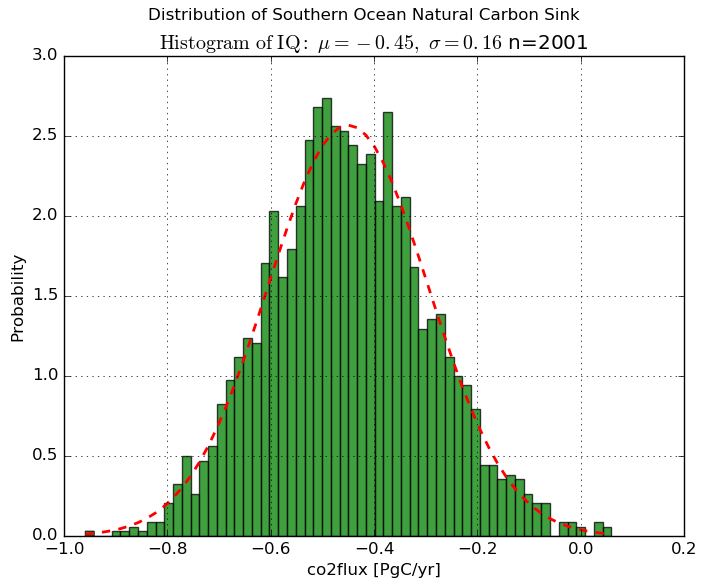
\includegraphics[scale=.4]{SOCS_temporal_gaussian.png} % from gfx folder
	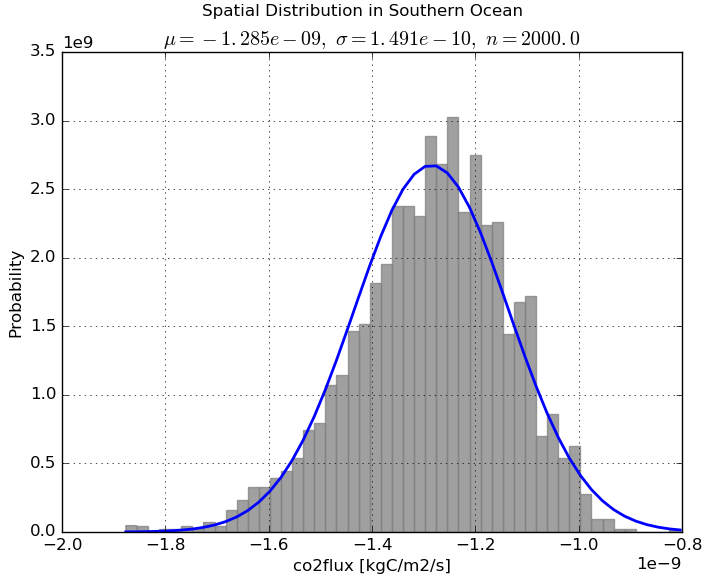
\includegraphics[scale=.4]{SOCS_spatial_gaussian.png} % from gfx folder
	\caption{Southern Ocean carbon sink: yearmean fieldsum 35-90S (left) and yearmean in a random grid cell (right)}
	\label{fig:SOCS_temporal_gaussian}
\end{figure}


\clearpage
\subsection{CO$_2$ flux trends}

\begin{figure}[h]
	\includegraphics[scale=.75,angle=0,trim=1.4cm 1.3cm 1cm 1cm,clip]{heatmap_not_de-ens-trended.pdf} % from gfx folder
	%\includegraphics[scale=.64,angle=90,trim=1.3cm 1.3cm 5cm 1cm,clip]{heatmap_de-ens-trended.pdf} % from gfx folder
\caption{Southern Ocean carbon sink trends per trendlength}
	\label{fig:heatmap}
\end{figure}

\begin{figure}[h]
	%\includegraphics[scale=.75,angle=0,trim=1.4cm 1.3cm 1cm 1cm,clip]{heatmap_not_de-ens-trended.pdf} % from gfx folder
	\includegraphics[scale=.75,angle=0,trim=1.4cm 1.3cm 1cm 1cm,clip]{heatmap_de-ens-trended.pdf} % from gfx folder
\caption{Southern Ocean carbon sink trends per trendlength; corrected for forced trend}
	\label{fig:heatmap_detrended}
\end{figure}



\clearpage
\subsection{Model evaluation additum}
\begin{figure}[h!]
	\centering
	\includegraphics[scale=.85,page=2,trim=1.8cm 13.3cm .8cm 6.5cm,clip]{Overview_SO_nutrient_comparison.pdf} % surf DIC
	\caption{Spatial distribution of the climatology of surface DIC (left) compared with GLODAPv2 data \citep{WOA2013} (right)}
	\label{fig:SOCS_comp_DIC}
\end{figure}



\begin{figure}[h!]
	\centering
	\includegraphics[scale=.85,page=1,trim=1.8cm 13.3cm .8cm 6.5cm,clip]{Overview_SO_nutrient_comparison.pdf} % phosph
	\caption{Spatial distribution of the climatological ensemble mean surface phosphate from 1980 to 2004 (left) compared with World Ocean Atlas (WOA) climatological data \citep{WOA2013} (right)}		
	\label{fig:SO_comp_phosph}
\end{figure}

\begin{figure}[h!]
	\centering
	\includegraphics[scale=.85,page=2,trim=1.8cm 13.3cm .8cm 6.5cm,clip]{Overview_SO_MPIOM_comparison.pdf} % zmld
	\caption{Spatial distribution of the ensemble mean climatology (1980-2004) of the sea-surface temperature (SST) (left) compared with WOCE climatology}
	\label{fig:SO_comp_sst}
\end{figure}

\clearpage
\subsection{Trends Additum}
\begin{figure}[h!]
	\centering
	\includegraphics[scale=1.6,trim=13.2cm 10.15cm 3.4cm 14.95cm,clip]{\memberpositive _positive_trend_8_obgc_overview_winter.pdf} %nutlimf
	\caption{Linear austral summer trends in sea-surface temperature (SST) for the case of the most positive monotonic 8-year CO$_2$ flux trend; hatched areas indicate where trends are outside the 5\% significance level}
	\label{fig:sst_pos}
\end{figure}

\begin{figure}[h!]
	\centering
	\includegraphics[scale=1.6,trim=13.2cm 10.15cm 3.4cm 14.95cm,clip]{\membernegative _positive_trend_8_obgc_overview_winter.pdf} %nutlimf
	\caption{Linear austral summer trends in sea-surface temperature (SST) for the case of the most negative monotonic 8-year CO$_2$ flux trend; hatched areas indicate where trends are outside the 5\% significance level}
	\label{fig:sst_neg}
\end{figure}


\clearpage
\subsection{Thermal separation by seasons}
\subsection{Positive CO$_2$ flux trend}
\begin{figure}[h!]
\centering
	\includegraphics[scale=.84,trim=7cm 15.7cm 7.8cm 6.4cm,clip]{\memberpositive _positive_trend_8_Landschuetzer_summer_overview.pdf}
	\includegraphics[scale=1.13,trim=8cm 5.6cm 6.8cm 17.8cm,clip]{\memberpositive _positive_trend_8_Landschuetzer_summer_overview.pdf}	
	\includegraphics[scale=1.7,trim=6cm 10.9cm 6cm 14cm,clip]{\memberpositive _positive_trend_8_Landschuetzer_summer_overview.pdf}
	\caption{Linear summer trends for the case of the most positive monotonic 8-year CO$_2$ flux trend; $\Delta$pCO$_2$ (a) and sea-level pressure \& winds (b); pCO$_{2,\text{thermal}}$ (c) and $\Delta$pCO$_{2,\text{non-thermal}}$ (d); hatched areas indicate where trends are outside the 5\% significance level}
	\label{fig:thermal_pos_summer}
\end{figure}

\begin{figure}[h!]
\centering
	\includegraphics[scale=.84,trim=7cm 15.7cm 7.8cm 6.4cm,clip]{\memberpositive _positive_trend_8_Landschuetzer_winter_overview.pdf}
	\includegraphics[scale=1.13,trim=8cm 5.6cm 6.8cm 17.8cm,clip]{\memberpositive _positive_trend_8_Landschuetzer_winter_overview.pdf}	
	\includegraphics[scale=1.7,trim=6cm 10.9cm 6cm 14cm,clip]{\memberpositive _positive_trend_8_Landschuetzer_winter_overview.pdf}
	\caption{Linear winter trends for the case of the most positive monotonic 8-year CO$_2$ flux trend; $\Delta$pCO$_2$ (a) and sea-level pressure \& wind vectors overlain as arrows (b); pCO$_{2,\text{thermal}}$ (c) and $\Delta$pCO$_{2,\text{non-thermal}}$ (d); hatched areas indicate where trends are outside the 5\% significance level}
	\label{fig:thermal_pos_winter}
\end{figure}

\clearpage
\subsection{Negative CO$_2$ flux trend}
\begin{figure}[h!]
\centering
	\includegraphics[scale=.84,trim=7cm 15.7cm 7.8cm 6.4cm,clip]{\membernegative _positive_trend_8_Landschuetzer_summer_overview.pdf}
	\includegraphics[scale=1.13,trim=8cm 5.6cm 6.8cm 17.8cm,clip]{\membernegative _positive_trend_8_Landschuetzer_summer_overview.pdf}	
	\includegraphics[scale=1.7,trim=6cm 10.9cm 6cm 14cm,clip]{\membernegative _positive_trend_8_Landschuetzer_summer_overview.pdf}
	\caption{Linear summer trends for the case of the most negative monotonic 8-year CO$_2$ flux trend; $\Delta$pCO$_2$ (a) and sea-level pressure \& wind vectors overlain as arrows (b); pCO$_{2,\text{thermal}}$ (c) and $\Delta$pCO$_{2,\text{non-thermal}}$ (d); hatched areas indicate where trends are outside the 5\% significance level}
	\label{fig:thermal_neg_summer}
\end{figure}

\begin{figure}[h!]
\centering
	\includegraphics[scale=.84,trim=7cm 15.7cm 7.8cm 6.4cm,clip]{\membernegative _positive_trend_8_Landschuetzer_winter_overview.pdf}
	\includegraphics[scale=1.13,trim=8cm 5.6cm 6.8cm 17.8cm,clip]{\membernegative _positive_trend_8_Landschuetzer_winter_overview.pdf}	
	\includegraphics[scale=1.7,trim=6cm 10.9cm 6cm 14cm,clip]{\membernegative _positive_trend_8_Landschuetzer_winter_overview.pdf}
	\caption{Linear winter trends for the case of the most negative monotonic 8-year CO$_2$ flux trend; $\Delta$pCO$_2$ (a) and sea-level pressure \& wind vectors overlain as arrows (b); pCO$_{2,\text{thermal}}$ (c) and $\Delta$pCO$_{2,\text{non-thermal}}$ (d); hatched areas indicate where trends are outside the 5\% significance level}
	\label{fig:thermal_neg_winter}
\end{figure}

\clearpage
\subsection{Misc}
\begin{figure}[h!]
\centering
	\includegraphics[scale=.8,trim=0.03cm 0cm 0cm 0cm,clip]{lighttemplimf.png}
	\caption{Combined light- \& temperature limitation function for the average phytoplankton growth rate in HAMOCC}
\label{fig:lighttemplimf}
\end{figure}
%https://tex.stackexchange.com/questions/85776/change-figure-numbering-for-appendix

\end{document}




















